\documentclass{article} % JASA requires 12 pt font for manuscripts
%\usepackage{JASA_manu}        % For JASA manuscript formatting

\usepackage{endfloat} % just for while I am writing

% for citations
\usepackage[authoryear]{natbib} % natbib required for JASA
\usepackage[dvips,colorlinks=true, citecolor=blue, linkcolor=blue]{hyperref}

%\definecolor{Blue}{rgb}{0,0,0.5}
\newcommand{\hh}[1]{{\color{orange} #1}}
\newcommand{\al}[1]{{\color{red} #1}}

% fonts
%\usepackage{kpfonts}

% for figures
\usepackage{graphicx}
\DeclareGraphicsExtensions{.eps, .pdf}
\graphicspath{{figures/}}

% help with editing and coauthoring
\usepackage{todonotes}
\newcommand{\alnote}[1]{\todo[inline,color=green!40]{#1}}

% title formatting
\usepackage[compact,small]{titlesec}

% page formatting
\usepackage[margin = 1in]{geometry}
\usepackage[parfill]{parskip}

% line spacing
\usepackage{setspace}
\doublespace

% For math typsetting
\usepackage{bm}
\usepackage{amstext}
\usepackage{amssymb}
\usepackage{amsmath}
\usepackage{amsfonts}
\usepackage{multirow}

% A few commands to make typing less tedious
\newcommand{\inv}{\ensuremath{^{-1}}}
\newcommand{\ginv}{\ensuremath{^{-}}}
\newcommand{\trans}{\ensuremath{^\prime}}
\newcommand{\E}{\ensuremath{\mathrm{E}}}
\newcommand{\var}{\ensuremath{\mathrm{Var}}}
\newcommand{\cov}{\ensuremath{\mathrm{Cov}}}


\title{Visual Inference for Linear Mixed-Effects Models}

\author{Adam Loy, Lendie Follett, Heike Hofmann, Dianne Cook\\
	Department of Statistics\\
	Iowa State University\\
	Ames, IA 50011-1210
}

\begin{document}
\maketitle
\begin{abstract}
Valid model-based statistical inference relies on proper specification of a model, making diagnostic tools central to analysis. Graphical methods are commonly used for checking the assumptions of a model; however, are often criticized as being too subjective, since decisions are based on one plot. This has lead to the reliance on conventional hypothesis tests to make formal decisions. Recently, visual inference has been established, providing a rigorous framework for graphical discovery that allows for the quantification of strength of evidence. In this paper we use visual inference as a framework to overcome common difficulties with conventional hypothesis tests and statistical graphics that are encountered in the selection and validation of linear mixed-effects models. Additionally, we compare three versions of Quantile-Quantile plots with respect to power.
\end{abstract}

%\tableofcontents
%------------------------------------------------------------------------------------
\section{Introduction}
%------------------------------------------------------------------------------------

Valid model-based statistical inference relies on proper specification of a model, making diagnostic tools central to analysis. Graphical methods are commonly used for checking the assumptions of a model. For example, in the linear model setting Quantile-Quantile (Q-Q) plots and scatterplots with smoothers are often used \citep{Cook:1999}.  
%In the Bayesian framework simulation from the posterior predictive distribution have been proposed to assess goodness-of-fit, which can displayed graphically \citep{Gelman:2004gg}. 
While the use of statistical graphics is wide-spread for model validation, graphics are often deemed too subjective to be the sole basis for model selection or validation. At the core of this criticism is the fact that decisions are being made based on a single plot. When a single plot is used, the detection of any unexpected structure in a plot leads to the conclusion that the model is inappropriate; however, artificial structures are often observed in the residual of properly specified complex models \citep[c.f.,][]{Morrell:2000ve, Gelman:2000dr}. These drawbacks lead to an over-reliance on conventional hypothesis tests %for model selection and validation 
in complex models where such procedures often perform sub-optimally.

%however, conventional practices for the selection and validation of linear mixed-effects models often rely on test statistics with questionable reference distributions and residual plots that exhibit artificial structure in well-fitting models. Graphical displays are often suggested 
%
%Recently, visual simulation-based diagnostics \citep{Gelman:2004gg} and inference \citep{Buja:2009hp} have been formulated, providing a rigorous framework for graphical discovery. Instead of relying on adjustments to reference distributions that must be considered on a case-by-case basis, we propose utilizing the framework of visual inference \citep{Buja:2009hp, mahbub:2013} as a unified graphical approach that harnesses our innate abilities to detect extremes to overcome such problems. This approach is able to enhance familiar statistical graphics from linear models, such as Quantile-Quantile (Q-Q) plots and scatterplots with smoothers, to avoid the detection of artificial structures. 

%Statistical modeling involves a cyclical process consisting of exploration, estimation, and validation. When a structure of interest is identified in the data we model this relationship and look past this structure in search of additional structure that is unexplained by the model; thus, exploratory and confirmatory methods in statistical modeling are inherently linked. While there is a wide-spread use of graphical methods for exploration, they are often deemed too subjective to be the sole basis for model selection or validation. This viewpoint leads to an over-reliance on conventional hypothesis tests 
%%for model selection and validation 
%in complex models where such procedures often perform sub-optimally.
%Until now, when such situations were encountered an analyst was forced to either accept the approximate results offered by conventional hypothesis tests or appeal to simulation via the parametric bootstrap to adjust results \citep[c.f.,][]{Longford:2001wy}. 
%\todo[inline]{what makes the parametric bootstrap solution unsatisfactory? -- we shouldn't bring it up unless there's a good reason to not use it. }
%\alnote{I refer to the fact that they require more computation time than the lineups later in the paper. Also, like classical hypothesis tests, they only provide decisions whereas lineups provide additional information.}
Recently, visual inference has been established \citep{Buja:2009hp, mahbub:2013}, providing a rigorous framework for graphical discovery that allows for the quantification of strength of evidence. Using visual inference, we suggest and validate a framework to overcome common difficulties with conventional hypothesis tests and statistical graphics that are encountered in the selection and validation of linear mixed-effects (LME) models. This approach is able to enhance familiar statistical graphics to avoid the detection of artificial structures. 



%In this paper we apply the  framework of visual inference  \cite{Buja:2009hp, mahbub:2013} to address common difficulties encountered in the selection and validation of linear mixed-effects (LME) models.

%Visual inference provides a unified graphical approach to account for such problems encountered with complex models while relying on familiar statistical graphics. 

In order to develop such graphical tools as complements to conventional tests, we must first define the inferential framework on which we rely.

%%------------------------------------------------------------------------------------
%\subsection{Visual inference}\label{sec:vi}
%%------------------------------------------------------------------------------------
%In order to develop graphical model diagnostics as substitutes for statistical tests of model assumptions, we must work within a rigorous inferential framework. 
%\cite{Gelman:2004gg} formulates a visual analog of simulation-based model diagnostics in which a visualization of an aspect of the model is compared to data generated under the model. \cite{Buja:2009hp} extend this idea, proposing two protocols that formalize a rigorous inferential framework for testing visual discoveries. In this section we outline the lineup protocol.

Classical statistical inference consists of 
\begin{enumerate}
	\item formulating a null and alternative hypothesis,
	\item calculating a test statistic,
	\item comparing the test statistic to a reference (null) distribution,
	\item and calculating a $p$-value on which we base our conclusion.
\end{enumerate}
Each of these steps has a direct analog in visual inference, as outlined by \cite{Buja:2009hp}. As we will apply visual inference for model diagnostics, we want to highlight these parallels in this framework: the null  hypothesis corresponds to some assumption about the model, such as e.g.~homogeneity of residual variance,
while
the alternative hypothesis encompasses any violation of this model assumption. For visual inference, the test statistic corresponds to a plot  that displays the model assumption and allows the observer to distinguish between scenarios under the null and alternate hypotheses. 
A plot of data generated consistently with the null hypothesis is called a null plot. The set of all null plots makes the reference distribution. 
If the model assumption holds, i.e.  under the null hypothesis, the plot of the observed data is indistinguishable from the null plots. 
In the lineup protocol the true plot is randomly embedded among a number of null plots.  

Figure~\ref{fig:fanned} gives a first example of a lineup. Each panel shows  line segments of different lengths  with varying slopes. 
Observers are asked to identify the plot that is the most different from the other plots.  What is your choice for the most different plot?  Any additional information is  withheld on purpose to prevent observers from (subconsciously)  introducing preconceived notions and making decisions that are not purely based on the data display. 

\begin{figure}
	\centering
	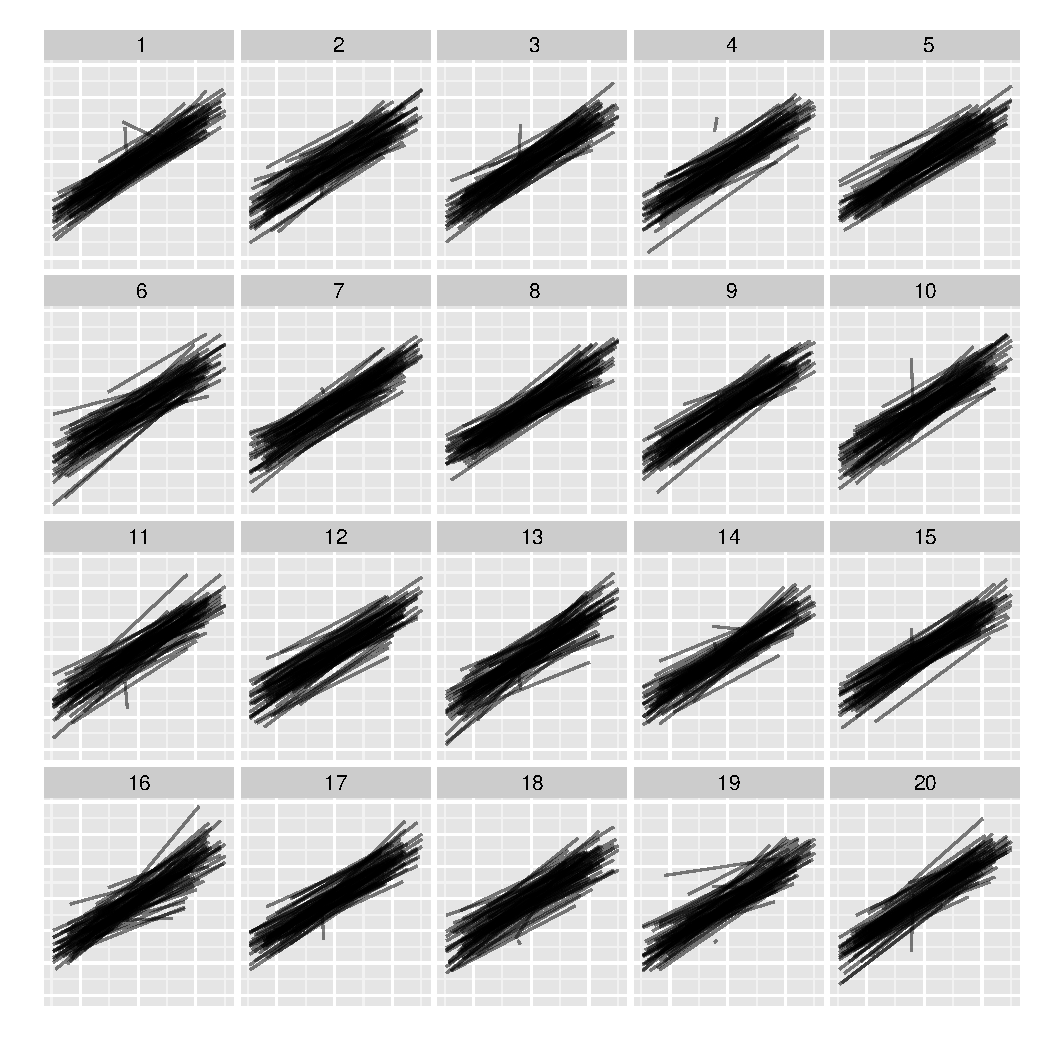
\includegraphics[width=\textwidth]{normexam_fanned_lineup16.pdf}
	\caption{\label{fig:fanned} Which plot is the most different from the other plots? What makes your plot different from the other plots?
	%Which is the real plot?
	}
\end{figure}


The lineup protocol allows for the estimation of a $p$-value associated with a lineup
based on an assessment  by human observers. Let $x$ be the number of observers, out of $N$, who chose the data plot from the lineup. The $p$-value is then the probability that at least $x$ observers choose the true plot, given that the true plot is not any different from the other plots in the lineup. Under the null hypothesis the probability for choosing the true plot is $1/m$, and $X$, the number of observers choosing the true plot, is distributed according to a Binomial distribution: $X \sim B_{N, p}$. The $p$-value is then estimated as
\begin{equation}\label{eqn.pvalue}
\widehat{p\text{-value}} = P(X \ge x) = \sum_{k= x}^N {N \choose k} \left(1/m\right)^k \left(1 - 1/m\right)^{N-k}.
\end{equation}

\hh{Based on XXX evaluations of Figure~\ref{fig:fanned}, XXX observers chose the true data from the lineup. This leads us to reject the null hypothesis that the data plot is consistent with the null model with a $p$-value of XXX. The actual model of the data and the null} \al{hypothesis?} \hh{are explained in detail in section~\ref{sec:select}. The data in this first lineup is shown in panel  $\sqrt{144} + 4$.}

The lineup protocol also allows for an assessment of the power of a lineup \citep{mahbub:2013}. 
%as the probability that in $N$ independent evaluations observers 
In $N$ independent evaluations, the probability that observers
choose the true plot more than $x_\alpha$ times is
\begin{equation}\label{eqn:power}
\widehat{\text{Power}} = \text{Power}_{N} = 1 - F_{X} (x_{\alpha}),
\end{equation}
where $F_X$ is the distribution of $X$ and $x_\alpha$ is the critical value for a given significance level of $\alpha$, i.e. $P(X >  x_{\alpha}) \le \alpha$. $X$ is composed of the sum of $N$ observers' (binary) decisions $X_i \sim B_{1, p_i}$, where  $p_i$ is the probability that individual $i$ chooses the true plot. This probability  depends both on the strength of the signal in the true plot and an individual's visual ability.
Assessing ability requires that an individual evaluates multiple lineups. If that is not possible, we have to assume that all individuals share the same ability, and the power calculation in eqn.~(\ref{eqn:power}) simplifies to $1 - B_{N, \hat{p}}(x_\alpha)$, where $\widehat{p}$ is an estimate for the probability that an individual chooses the true plot based on a specific lineup. Similar to classical inference, we can make use of power to assess sensitivity of tests. This allows us to make decisions about designs for particular tasks by evaluating lineups displaying different designs of the same data. An example of this is given in section~\ref{sec:qqplot}, where we compare three variations of the familiar Quantile-Quantile (Q-Q) plot \citep{Wilk:1968}.

Unlike classical hypothesis tests, visual inference allows us to also  collect information on what aspect of the display led each observer to their choice. 
%Rather than to just reject a null hypothesis 
This additional information helps us to assess more specifically, which part of the null hypothesis seems to be violated, something that is not provided in classical hypothesis tests. \hh{An example of this is shown in section XXX}


%\subsection{Model notation and formulation} 
%------------------------------------------------------------------------------------

Linear mixed-effects models are versatile models that allow for dependence that is expected when data are organized in groups.
%---such data structures are especially common in social science research where studies often focus on responses from human subjects. 
Examples of such structures include when individuals are naturally grouped by organization (e.g., students within schools), geography (e.g., voters within states), and interviewer (e.g., respondents assigned to an interviewer). The additional flexibility offered by these models to incorporate data at the observation-level and the group-level while allowing for dependencies between individuals within the same group complicates model exploration and validation. For example:
\begin{itemize}
\item Test statistics used for model selection and validation rely on asymptotic reference distributions which often perform poorly in finite sample situations. 
%Likelihood ratio tests for model selection are known to suffer from boundary effects, and while adjustments to the reference distributions have been proposed \citep{Stram:1994wd}, they do not hold in all cases.

\item Residual plots often display noticeable patterns that are artifacts of the model estimation procedure rather than indications of lack of fit. This problem is especially pronounced for plots of the predicted random effects \cite[c.f.,][]{Morrell:2000ve}.

\item The empirical distribution of the random effects often does not resemble the theoretical distribution rendering conventional use of normality tests and Quantile-Quantile plots ineffective for distributional assessment.
\end{itemize}

In this paper we consider the continuous response linear mixed-effects model
%
\begin{equation}\label{eq:hlm}
	\underset{(n_i \times 1)}{\bm{y}_i} = \underset{(n_i \times p)}{\bm{X}_i} \ \underset{(p \times 1)}{\bm{\beta}} + \underset{(n_i \times q)}{\bm{Z}_i} \ \underset{(q \times 1)}{\bm{b}_i} + \underset{(n_i \times 1)}{\bm{\varepsilon}_i}
\end{equation}
%
where $\bm{y}_i$ is the vector of outcomes for the $n_i$ level-1 units in group $i=1, \ldots, g$, $\bm{X}_i$ and $\bm{Z}_i$ are design matrices for the fixed and random effects, respectively, $\bm{\beta}$ is a vector of fixed effects governing the global mean structure, $\bm{b}_i$ is a vector of random effects governing the between-group covariance structure, and $\bm{\varepsilon}_i$ is a vector of level-1 error terms governing the within-group covariance structure. We further assume that the random effects are a random sample from $\mathcal{N}(\bm{0},\ \bm{D})$ and are independent from the level-1 error terms, which we assume are a random sample from $\mathcal{N}(\bm{0},\sigma^2 \bm{I})$. %\bm{R}_i)$. 
Inference typically centers around either the marginal or conditional distribution of $\bm{y}_i$, depending whether global or group-specific questions are of interest.
Based on model \eqref{eq:hlm} the marginal distribution of $\bm{y}_i$ is given by
%
\begin{equation}\label{eq:marginalmod}
\bm{y}_i \sim \mathcal{N}\left(\bm{X}_i\bm{\beta},\ \bm{V}_i \right)
\end{equation}
%
where $\bm{V}_i = \bm{Z}_i \bm{DZ}_i + \sigma^2 \bm{I}_i$, and the conditional distribution of $\bm{y}_i$ given $\bm{b}_i$ is given by
%
\begin{equation}\label{eq:conditionalmod}
\bm{y}_i | \bm{b}_i \sim \mathcal{N}\left(\bm{X}_i\bm{\beta} + \bm{Z}_i \bm{b}_i, \ \bm\sigma^2 \bm{I}_i \right)
\end{equation}
%



As with the classical linear model with uncorrelated errors, residuals are central to the exploration of a linear mixed-effects model. For linear mixed-effects residual analysis is complicated by the fact that there are numerous quantities that can be defined as \emph{residuals}, with each residual quantity being associated with different aspects of the model. Two fundamental residuals for model checking include
%
\begin{itemize}
\item the level-1 residuals (i.e., the conditional residuals or error terms) $\widehat{\bm{\varepsilon}}_i = \bm{y}_i - \bm{X}_i \widehat{\bm{\beta}} - \bm{Z}_i \widehat{\bm{b}}_i$,

\item and the level-2 residuals (i.e., the predicted random effects) $\widehat{\bm{b}}_i$
\end{itemize}
%
where, assuming $\bm{V}$ is known,
\begin{equation}\label{eq:glsb}
	\widehat{\bm{\beta}} = 
	\left(\sum^m_i \bm{X}\trans_i \bm{V}^{-1}_i \bm{X}_i \right)^{-1} 
	\sum^m_i \bm{X}_i\trans \bm{V}_i\inv \bm{y}_i,
\end{equation}
and
\begin{equation}\label{eq:eb}
	\widehat{\bm{b}}_i = \bm{D} \bm{Z}_i\trans \bm{V}_i^{-1} 
	\left(\bm{y}_i - \bm{X}_i \widehat{\bm{\beta}} \right)
\end{equation}
%
In practice $\bm{V}$ is unknown, so estimates for $\bm{D}$ and $\bm{V}$ are used in the above equations. These estimates are commonly found through maximum likelihood (ML) or restricted maximum likelihood (REML). Lineups for visual inference heavily rely on the types of residuals defined above. %Next, we compare conventional and visual inference for model selection and validation.
%Below we discuss methods commonly used to check the validity of the assumptions made on model \eqref{eq:hlm} using the level-1 and -2 residuals.


Throughout this paper we discuss visual inference in the framework of linear mixed-effects models and suggest  graphical tests in situations where the assumptions of conventional inference are violated. In Section~\ref{sec:select} we focus on model building. In section~\ref{sec:checking} we present graphical tests for model validation. We also show results of a study investigating the power of three different versions of the familiar Q-Q plot. 

%\todo[inline]{paragraph on the structure of the paper:  next section deals with visual inference in the framework of hierarchical models, and suggests a series of visual tests as alternative to tests that in the classical setting don't work too well because of easily violated assumptions or nature of the setup. Then we will discuss using power to choose specific designs in the evaluation of distributional assumptions in the familiar graphical setting of the Q-Q plots. }



%------------------------------------------------------------------------------------
\section{Model selection}\label{sec:select}
%------------------------------------------------------------------------------------

%The lineup protocol presents a unified approach to overcome the difficulties encountered when checking the validity of a hierarchical linear model. The only change necessary to utilize this approach to model checking is the generation of null plots, for which we use the parametric bootstrap. Consequently, the ``standard'' residuals plots can be used within this framework in order to overcome the subjectiveness of interpretation and identification of artificial structures, making visual inference a natural extension of conventional model checking. 
%In this section we discuss several examples of lineups that we have found useful for model checking; however, we do not intend to present an exhaustive overview.

%In this section we discuss how visual inference can be used during model selection.
One statistical model is nested within another when the \emph{larger model} contains all components included in the \emph{smaller model}
% with respect to both fixed and random effects, 
 as well as some additional component(s). For example, the larger model may include additional fixed effects, or include additional random effects. Two are not nested when one model, previously termed the smaller model, is not a special case of the other. For example, if two models contain different sets of fixed effects.
 Model selection for linear mixed-effects models relies on the comparison of nested models for the selection of both the fixed and random components of the model. To select fixed effects $t$- and $F$-tests are commonly used, while likelihood ratio tests are used to select the random effects. In this section we discuss how to use visual inference as a unified testing framework for model selection for both nested and non-nested models.


%\subsubsection{Conventional practices}
\subsection{Comparing nested models}\label{sec:select-fixed}
%------------------------------------------------------------------------------------

It is standard practice to use a $t$-test, $F$-test, or likelihood ratio test to determine whether a fixed effect describes a significant portion of the unexplained variability in a linear mixed-effects model. Likelihood ratio tests are more generally applicable in comparing nested models, but are most commonly in the selection of random effects. 
%One statistical model is nested within another when the \emph{larger model} contains all components included in the \emph{smaller model}, with respect to both fixed and random effects, as well as some additional component(s). For example, the larger model could differ by including additional fixed effects, or by including additional random effects. 
While statistical software has made performing many of these tests easy, situations often arise that complicate such tests. Below we outline such situations.

\begin{description}
\item[\bf Fixed effects: ] Likelihood ratio tests based on REML estimation cannot be used to test different fixed effects structures. Maximum likelihood estimation allows for such comparisons, but is anti-conservative. 
\item[\bf Random components: ] When the covariance parameter being tested lies on the boundary of the parameter space, the asymptotic distribution of the likelihood ratio is no longer a $\chi^2$ distribution. Approximations have been suggested and shown to be useful in many situations \citep{Stram:1994wd, Morrell:1998ua}, but no one approximation holds for all situations leading to either conservative or anti-conservative decisions. 
\end{description}


Visual inference provides an alternative to conventional hypothesis tests that does not require different rules based on the method of estimation or location of a parameter in the parameter space. Rather, visual inference depends on the choice of an appropriate plot highlighting the aspect of the model in question, the number of null plots, and the number of independent observers. Below we discuss how visual inference can be utilized to test the significance of fixed and random effects.

\paragraph{Fixed effects.} To test the significance of a fixed effect, we suggest using a plot comparing a residual quantity from the model without the variable of interest with the values of that variable. 
The residual used depends on the level at which the variable of interest enters the model: if the variable enters at the observation-level (level-1), then the level-1 residuals are used; if the variable enters at the group level, then both the level-1 and level-2 residuals are explored as the variable has the potential to explain additional variation at either level of the model.
Additionally, the type of plot depends on the variable type---if a continuous variable is targeted,  a scatterplot with a smoother is suitable for testing; for a discrete covariate, we make use of side-by-side boxplots. 
In this setting, the null plots are generated using the parametric bootstrap  with a model that omits the variable of interest. The true plot is constructed from the same model but using the observed data. 

\begin{figure}[h]
	\hfill
	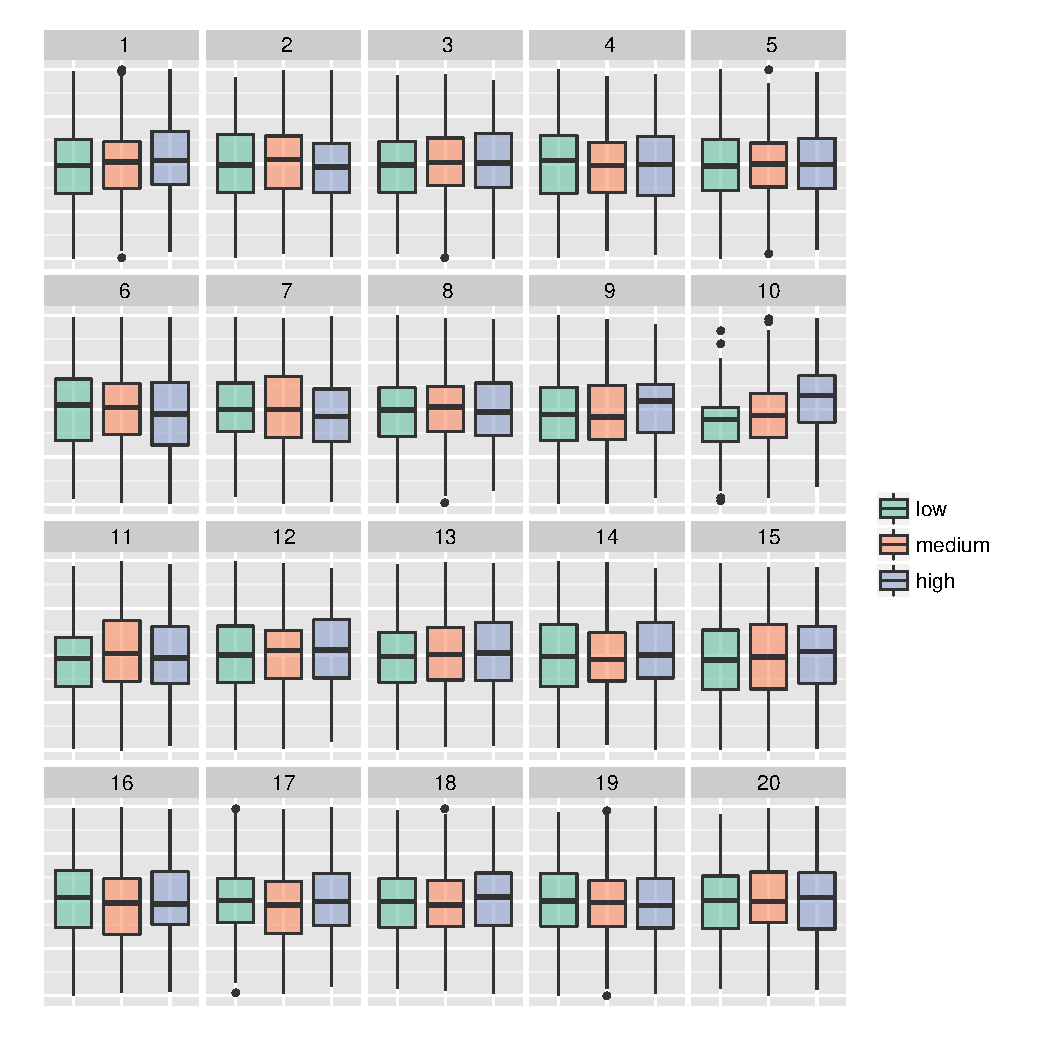
\includegraphics[width=0.9\textwidth]{autism_sicdegp_level1_lineup10.pdf}
	\caption{\label{fig:boxplot-ordered} 
%	\todo[inline]{I'm starting to get nitpicky again :)
%	The legend is added (to make the point later that it doesn't help much with the overall pattern), the boxes are a bit transparent (maybe alpha of 0.6?) so the gridlines in the back don't completely disappear and we need to use a different color scheme - the red and the green are not color blind safe. } 
%	\todo[inline]{Why did you decide to remove the outliers? Are you worried the outliers distract from the pattern? - We could test that!}
%	\alnote{That is why I removed the outliers. It would be interesting to test.}
	Which of the plots is the most different? Which feature led you to your choice?} 
\end{figure}

Figure~\ref{fig:boxplot-ordered} illustrates the use of this type of lineup. In our study, XXX observers were asked to choose the plot that is the most different from the rest. XXX of them identified the data plot (panel $2^3 + 2$), corresponding to a $p$-value of XXX, with XXX\% pointing to the trend as distinguishing feature. 
This lineup is chosen
to determine whether a child's language development at age 2 (low, medium, or high) helps explain the development of social skills from childhood to adolescence for children diagnosed with autism spectrum disorder. Displayed on the $y$-axis are level-1 residuals from a longitudinal model. Clearly, language development at age 2 accounts for a significant amount of the remaining residual variability.
%The underlying data are level-1 residuals from a longitudinal 
%Lineup testing for the significance of social skills (low, medium, or high) for a longitudinal model investigating investigating the development of social skills from childhood to adolescence for children diagnosed with autism spectrum disorder. Here the level-1 residuals are used to see if the variable accounts for any additional residual variability. 


%\begin{figure}
%	\hfill
%	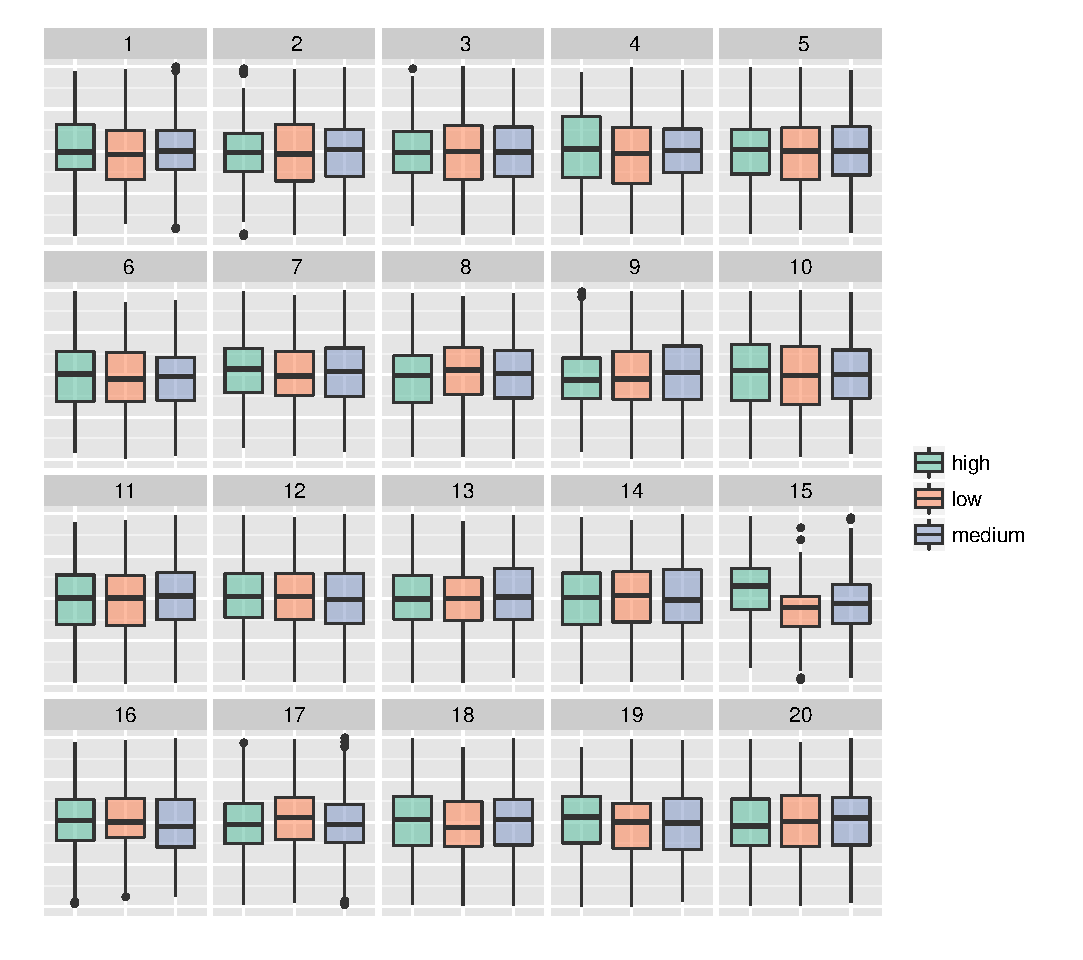
\includegraphics[width=0.9\textwidth]{autism_sicdegp_level1_lineup4.pdf}
%	\caption{\label{fig:boxplot-unordered} Lineup testing for the significance of social skills (low, medium, or high) for a longitudinal model investigating investigating the development of social skills from childhood to adolescence for children diagnosed with autism spectrum disorder. Here the level-1 residuals are used to see if the variable accounts for any additional residual variability. Which is the real plot?}
%\end{figure}


\paragraph{Random effects.} Tests of the random part of a hierarchical model focus on two questions: (1) whether a marginal random effect improves the model and (2) whether allowing the random effects to be correlated improves the model. Different plots must be used to answer each question. To answer the first question, we suggest using plots comparing the response and the explanatory variable of interest using appropriate (often linear) smoothers for each group. Scatterplots comparing the predicted random effects can be used to answer the second question.

The lineup in Figure~\ref{fig:fanned} is chosen to test the relationship between scores from the General Certificate of Secondary Education Exam (GCSEE) and the  standardized London Reading Test (LRT).  Each line segment represents one of 65 inner-London schools. The slope of each line is determined by a linear regression \al{relating} the two test scores for all students at a school. 
The question of interest is whether random slopes for LRT scores are required to  represent the relationship between GCSEE and LRT scores ($H_1$). Correspondingly, data for the null plots  is  created by simulating GCSEE scores from a model with only a single random effect, the random intercept.
The resulting scores for each school are regressed on LRT results and shown as lines.
%\al{and overlaying linear smoothers for each school.}
%Revisiting Figure~\ref{fig:fanned} we see an example of testing for the inclusion of a random effect. Recall that the initial model was a random intercept model using a student's score on the standardized London Reading Test to describe their age 16 score on the General Certificate of Secondary Education examination.
 %To construct this figure we used the parametric bootstrap to generate simulated GCSEE exam scores, fit separate regression models to the simulated responses, and then plotted the fitted model for each school. 
 If the model is appropriate, then the overall pattern of the lines in the null plots should resemble the observed data. In this example, we find that the true plot (panel $\sqrt{144} -2$) is identifiable \hh{as XXX of the XXX observers pick the data plot. The main comment for their choice was a larger ``fanning out'' of the line segments in the plot. This is consistent with a larger variance of slopes than the null model allows;}
  %GCSEE scores   for higher scores on the standardized LRT than \hh{accommodated for} in the null plots; 
  thus, we find evidence supporting the inclusion of a random slope for standardized LRT. This conclusion agrees with the results of the likelihood ratio test, and did not require the use of an asymptotic distribution to calculate the $p$-value.

Having considered the value of a random slope in the model, we next consider whether the model needs to allow the random effects to be correlated ($H_1$). While this is an example of a standard likelihood ratio test problem---a correlation of zero is not on the boundary of the parameter space---using a lineup keeps all tests of the random effects in a unified framework. The lineup in Figure~\ref{fig:ranef-corr} shows scatterplots of the predicted random effects with overlaid regression lines. This type of plot is suggested by  \cite{Morrell:2000ve} as a visual diagnostic for assessing the amount of correlation. 
 The null plots in the lineup are created by simulation from the model that does not allow for correlation between the random effects, and the true plot is created using the predicted random effects from a model allowing for correlation between the random effects.
The slopes of the regression lines are indicative of the amount of correlation. Note that with a higher amount of shrinkage in the random effects we start to see more lines with a higher amount of slope. 
 If the correlation between the random effects is not necessary, then the true plot will display little correlation and be indistinguishable from the null plots.
 \hh{The lineup allows us to gauge the amount of correlation between the random effects while accounting for the effect of shrinkage in the model.}
  In Figure~\ref{fig:ranef-corr} the true plot (panel~$2 + \sqrt{25}$) was identified \al{by XXX of the XXX observers}, providing evidence supporting the inclusion of the additional parameter.

\begin{figure}
	\centering
	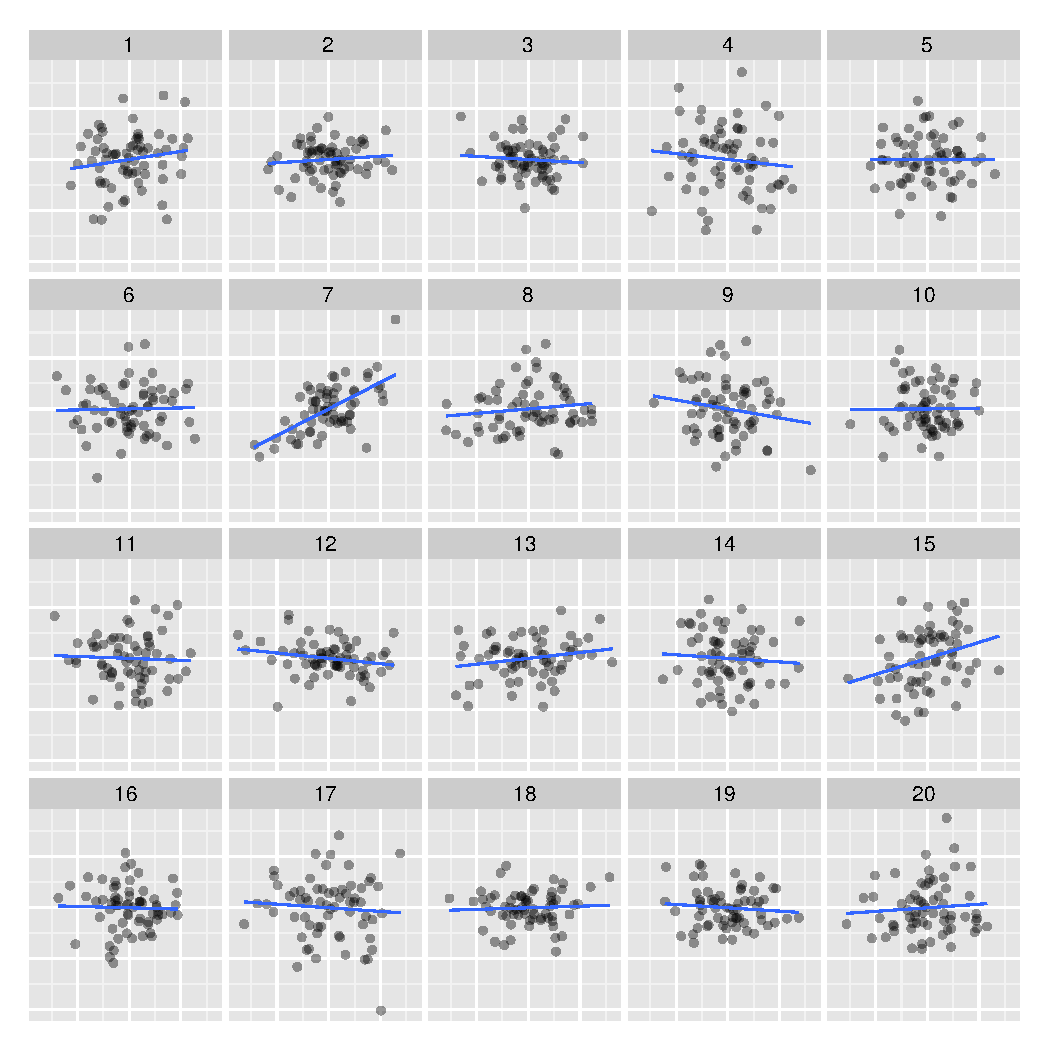
\includegraphics[width=\textwidth]{exam_corr_lineup7.pdf}
	\caption{\label{fig:ranef-corr} Lineup for testing correlation between random effects. Which plot is the most different of the others? What feature in the panel led you to your choice? }
\end{figure}

%\alnote{We could move the negative lineups that we did not include in the study to the appendix. I am thinking about this more from the perspective of when we submit to a journal with length restrictions}
%
%\begin{figure}
%	\centering
%	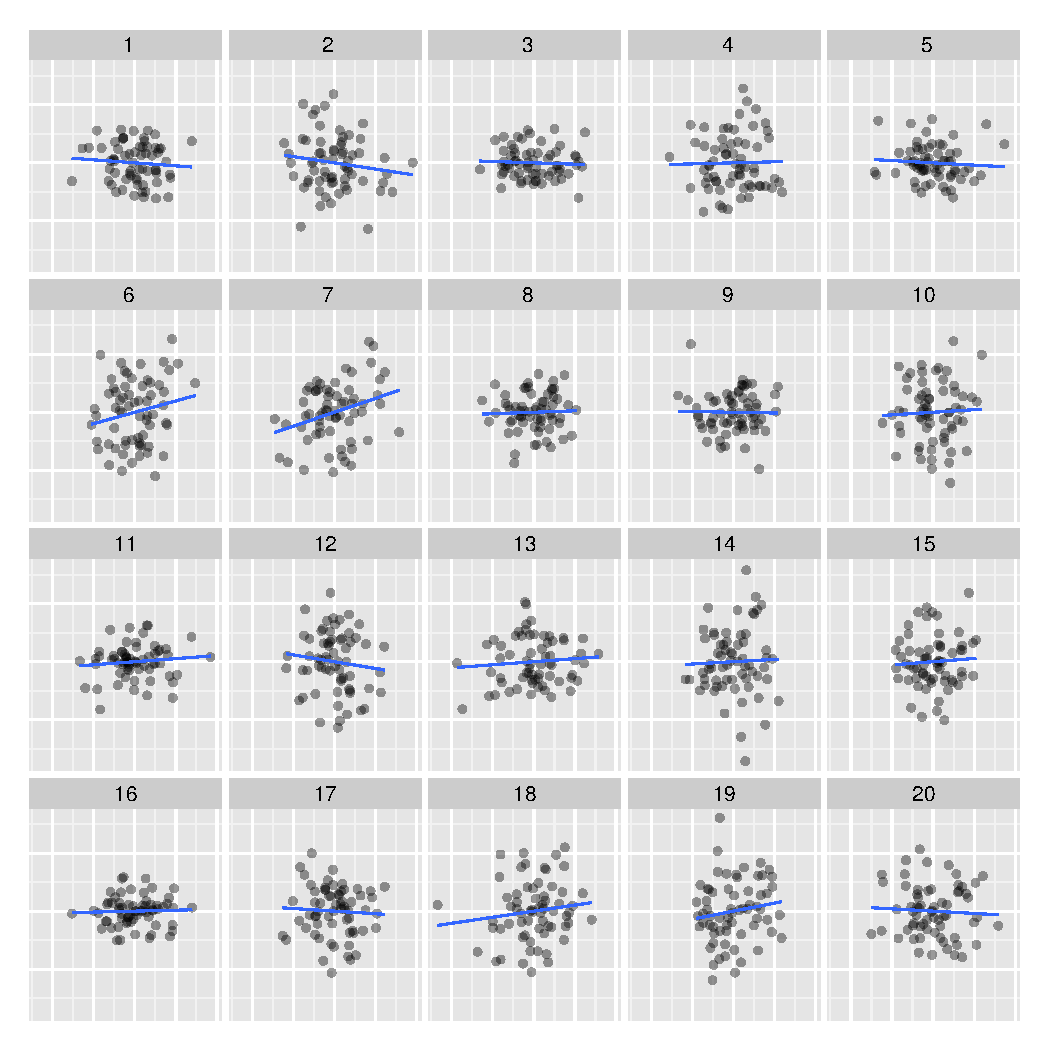
\includegraphics[width=\textwidth]{normexam_uncorr_lineup13.pdf}
%	\caption{\label{fig:ranef-uncorr}  Lineup testing the need to allow for correlation between the two random effects. These 20 plots compare the predicted random intercept and slope for the model fit to the Exam data. Which is the real plot?}
%\end{figure}


%\todo[inline]{Make the following paragraph a bullet list. This will help to emphasize the important parts. At the moment they get lost a bit.
%\begin{description}
%\item[\bf Fixed effects in nested models: ] likelihood ratio tests based on REML estimation do not allow for testing different fixed effect structures. Maximum likelihood estimation allows for it, but is conservative. 
%\item[\bf Random components in nested models: ] likelihood ratio tests for random components suffer from boundary effects. 
%\end{description}}

%Statistical software has made performing $t$-tests for fixed effects simple, but more thought is often required when performing a likelihood ratio test. More specifically, likelihood ratio tests can only be used with nested models fit by REML if they differ only with respect to their random components. This is because the restricted log likelihood contains a term that changes with $\bm{X}_i$ \citep[c.f.,][Section 2.2.5]{Pinhiero:2000vf}. Nested models fit by ML do not have this restriction, so likelihood ratio tests can be used to test both the fixed and random effects. 
%Additional complications arise in the computation of a $p$-value for the likelihood ratio test for covariance parameters on the boundary of the parameter space. In this case, the asymptotic reference distribution is not $\chi^2$ with degrees of freedom equal to the difference in the number of parameters. \cite{Stram:1994wd} suggest the use of a 50:50 mixture of $\chi^2$ distributions with $q$ and $q + 1$ degrees of freedom when testing $q$ versus $q + 1$ random effects. While this approximation has been shown to be useful \citep{Morrell:1998ua}, it does not apply to every case.  We refer the reader \citet[Section 2.4.1]{Pinhiero:2000vf} for an example of when a this approximation is not successful. The lack of a general rule for approximating the distribution of the likelihood ratio test statistic reveals the need for a more transparent procedure for determining whether a random effect should be included in the model.


\subsection{Comparing non-nested models}
%------------------------------------------------------------------------------------
If two models are not nested, then the likelihood ratio test cannot be used to determine the preferred model. In this case, it is conventional practice to use the Akaike Information Criterion (AIC) as an index enabling model comparison, where the model with the smaller AIC is preferred. While AIC provides a concise and convenient way to compare non-nested models, it is only an index and does not address whether the model with the smaller AIC is significantly ``better'' than the other. To do this, we propose using lineups to investigate the goodness-of-fit of each model. If inadequacies are discovered in one model but not in the other, then this supports the use of the properly specified model. This approach is similar in concept to comparing the AIC from each model, but by focusing on an investigation of how the true data depart from the assumptions made by the model we can see why a model is preferred.


%\subsubsection{Proposals for visual inference}\label{model-selection}
%------------------------------------------------------------------------------------

%Visual inference provides an alternative to conventional hypothesis tests that does not have limitations based on whether ML or REML was used to fit the model since it does not rely on the (restricted) log likelihood. Additionally, the $p$-value from a visual test is calculated using the Binomial distribution, which does not require adjustments to an asymptotic distribution. Rather, visual inference depends on the plot chosen, the number of alternatives, and the number of viewers. Below we discuss plots for visual inference useful in model selection.

%\paragraph{Fixed effects.} To test the significance of a fixed effect, we suggest using a plot comparing a residual quantity from the model without the variable of interest and the values of that variable. The residual that should be used depends on the level at which the variable of interest enters the model---if the variable enters at the observation-level (level-1), then the level-1 residuals should be used; if the variable enters at the group level, then both the level-1 and level-2 residuals should be explored as additional variation at either level could be explained by this variable. Additionally, the type of plot depends on the variable type---if a continuous variable is targeted,  a scatterplot with a smoother \hh{is suitable for testing}; for a discrete covariate, \hh{we can make use of} side-by-side boxplots. 
%
%
%In this setting, the null plots are generated using the parametric bootstrap with a model that omits the variable of interest. The true plot is constructed from the same model but using the observed data. Figure~\ref{fig:boxplot-ordered} illustrates the use of this type of lineup to determine whether a child's language development at age 2 (low, medium, or high) helps explain the development of social skills from childhood to adolescence for children diagnosed with autism spectrum disorder. Which is the real plot? 
%
%\begin{figure}
%	\centering
%	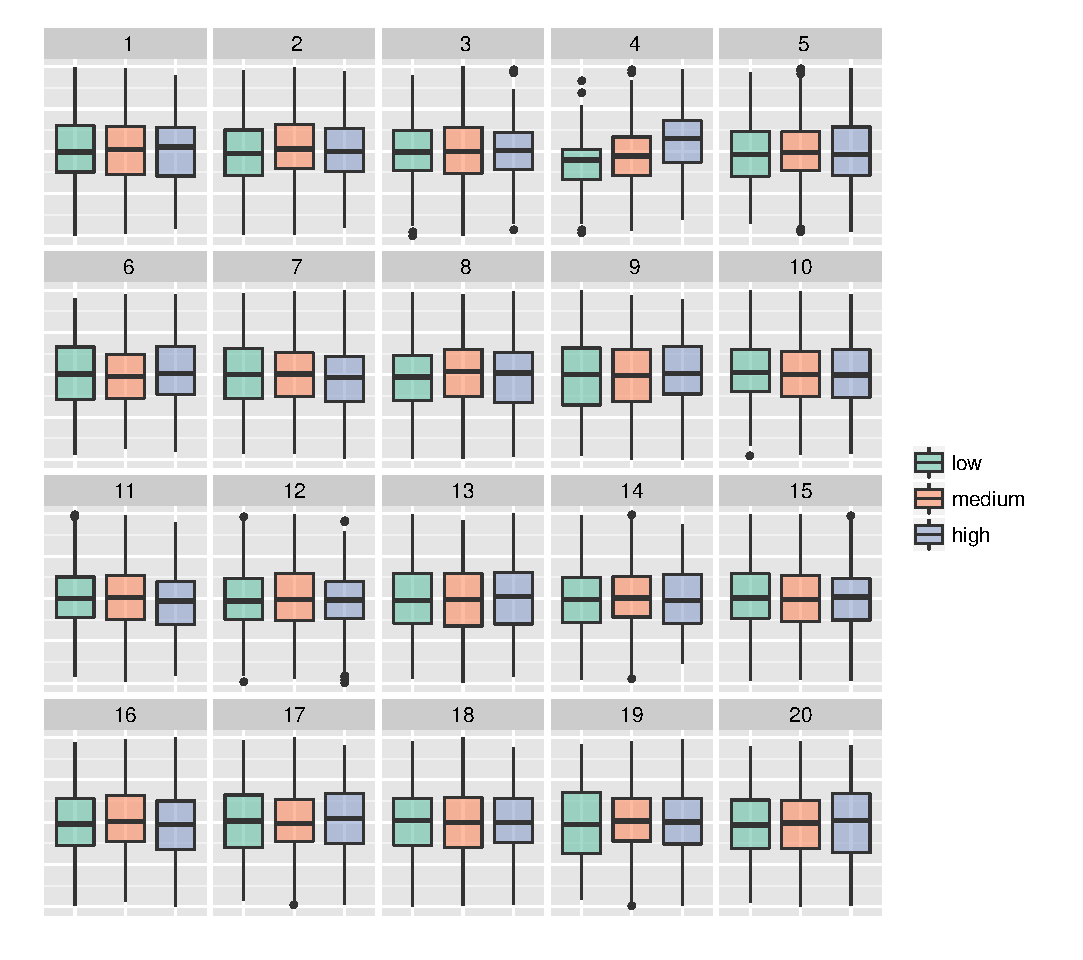
\includegraphics[width=\textwidth]{autism_sicdegp_level1_lineup5.pdf}
%	\caption{\label{fig:boxplot-ordered} Lineup testing for the significance of social skills (low, medium, or high) for a longitudinal model investigating investigating the development of social skills from childhood to adolescence for children diagnosed with autism spectrum disorder. Here the level-1 residuals are used to see if the variable accounts for any additional residual variability. Which is the real plot?}
%\end{figure}
%
%\todo[inline]{I also included the unordered boxplots so we could look at the difference}
%
%\begin{figure}
%	\centering
%	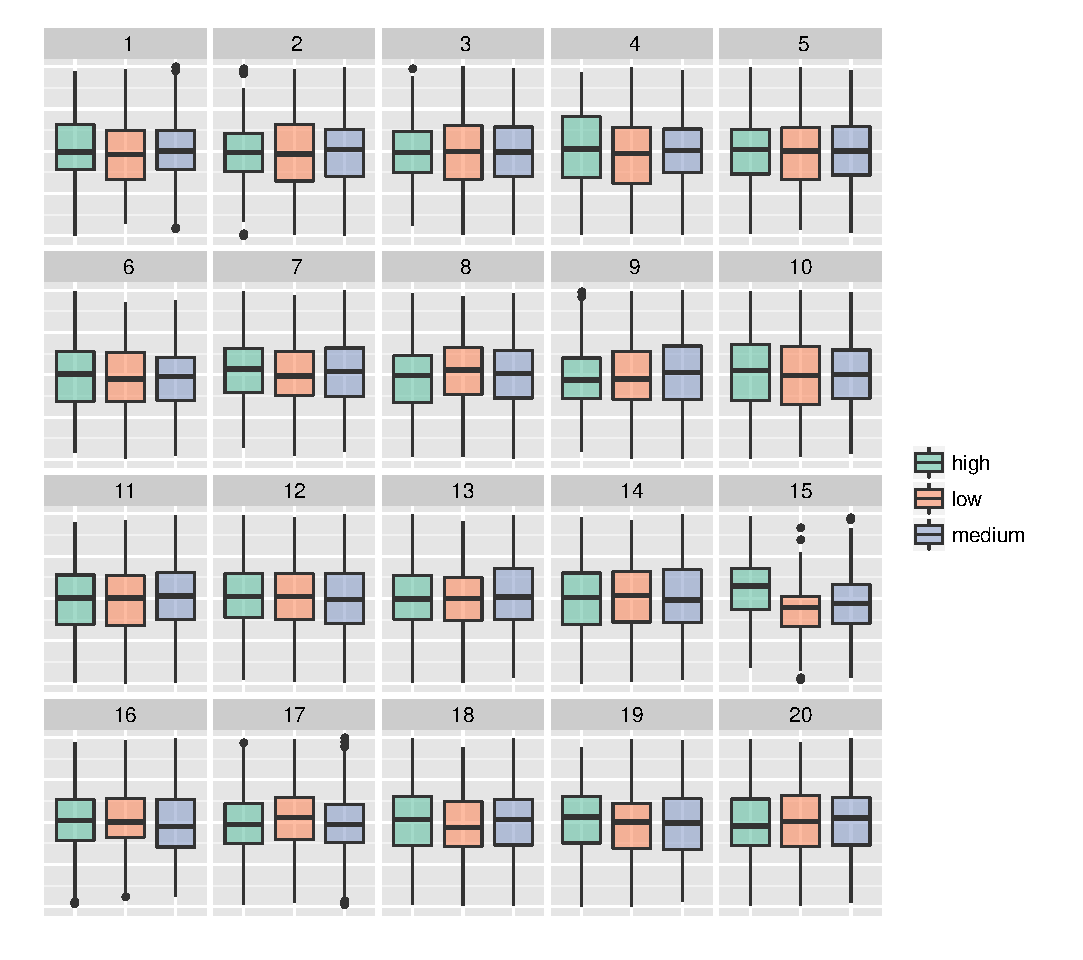
\includegraphics[width=\textwidth]{autism_sicdegp_level1_lineup4.pdf}
%	\caption{\label{fig:boxplot-unordered} Lineup testing for the significance of social skills (low, medium, or high) for a longitudinal model investigating investigating the development of social skills from childhood to adolescence for children diagnosed with autism spectrum disorder. Here the level-1 residuals are used to see if the variable accounts for any additional residual variability. Which is the real plot?}
%\end{figure}

%To illustrate the use of visual tests for fixed effects...\todo{Choose a data set!}


%\paragraph{Random effects.} Tests of the random part of a hierarchical model focus on two questions: (1) whether a marginal random effect improves the model and (2) whether allowing the random effects to be correlated improves the model. Different plots must be used to answer each question. To answer the first question, we suggest plots comparing the response and the explanatory variable of interest using appropriate (often linear) smoothers for each group. Scatterplots comparing the predicted random effects can be used to answer the second question.
%
%\hh{The lineup in figure~\ref{fig:fanned} is chosen to test the relationship between scores from the General Certificate of Secondary Education exam (GCSEE) and the  standardized London Reading Test (LRT).  Each line segment represents one of 65 inner-London schools. The slope of each line is determined by a linear regression of the two test scores for all students at a school. 
%The question of interest is whether random slopes for LRT scores are required to  represent the relationship between GCSEE and LRT scores ($H_1$). Correspondingly, data for the null plots  is  created by simulating GCSE exam scores from a model with a random intercept only.}
%\hh{The resulting scores for each school are regressed on LRT results and shown as lines} 
%%\al{and overlaying linear smoothers for each school.}
%
%
%%
%%Revisiting Figure~\ref{fig:fanned} we see an example of testing for the inclusion of a random effect. Recall that the initial model was a random intercept model using a student's score on the standardized London Reading Test to describe their age 16 score on the General Certificate of Secondary Education examination.
% %To construct this figure we used the parametric bootstrap to generate simulated GCSEE exam scores, fit separate regression models to the simulated responses, and then plotted the fitted model for each school. 
% If the model is appropriate, then the \hh{overall pattern of the lines in the null plots} should resemble the observed data. In this example, we find that the true plot (panel $\sqrt{144} + 1$) is identifiable 
%  \todo[inline]{we don't know that the true panel is identifiable, we do need to wait for the results first.}
%  \todo[inline]{true. I suppose I was just writing with an expected outcome in mind.}
%  as the variance of GCSEE scores is larger for higher scores on the standardized LRT than in the null plots; thus, we find evidence supporting the inclusion of a random slope for standardized LRT. This conclusion agrees with the results of the likelihood ratio test, and did not require the use of an asymptotic distribution to calculate the $p$-value.
%
%Having considered the value of a random slope in the model, we next consider whether the model needs to allow the random slope and intercept to be correlated ($H_1$). While this is an example of a standard likelihood ratio test problem, as a correlation of 0 is not on the boundary of the parameter space, a using a lineup keeps tests of the random effects in a unified framework. The lineup in Figure~\ref{fig:ranef-corr} shows scatterplots of the predicted random effects with a linear smoother. The null plots are created by simulation from the model that does not allow for correlation between the random effects, and the true plot is created using the predicted random effects from a model allowing for correlation between the random effects. If the correlation between the random effects is not necessary, then the true plot will display little correlation and be indistinguishable from the null plots. In Figure~\ref{fig:ranef-corr} the true plot (panel $\sqrt{70 + 11}$) is easily identified, providing evidence supporting the inclusion of the additional parameter.
%
%\begin{figure}
%	\centering
%	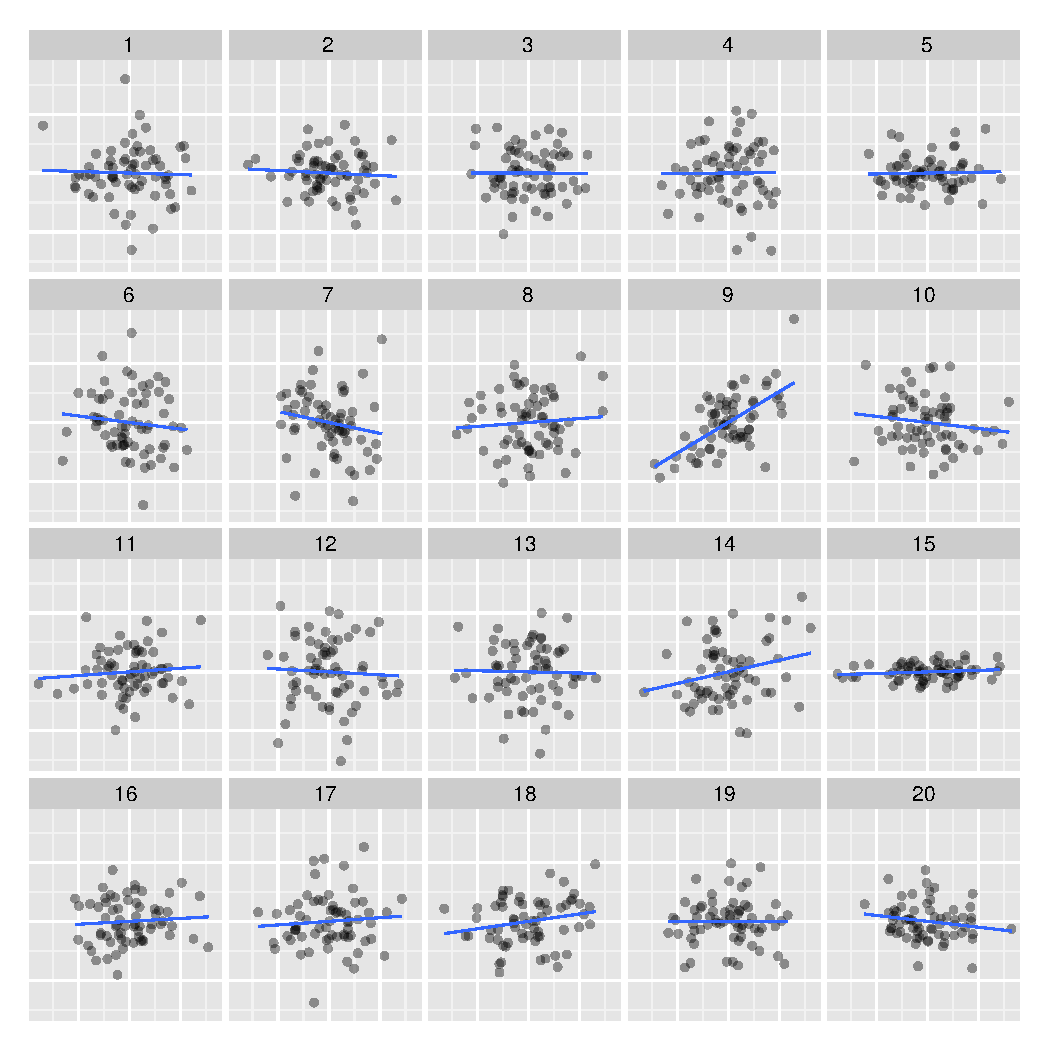
\includegraphics[width=\textwidth]{normexam_corr_lineup9.pdf}
%	\caption{\label{fig:ranef-corr} Lineup testing the need to allow for correlation between the two random effects. These 20 plots compare the predicted random intercept and slope for the model fit to the Exam data. Which is the real plot? Note that this is the type of plot that \cite{Morrell:2000ve} discussed. If there were a higher degree of shrinkage in the random effects we would start to see more false lines in these plots, but as it is, if you remove the smoother and use $\alpha$-blending a line/curve is visible consisting of the random effects of children with only one observation.}
%\end{figure}
%
%\begin{figure}
%	\centering
%	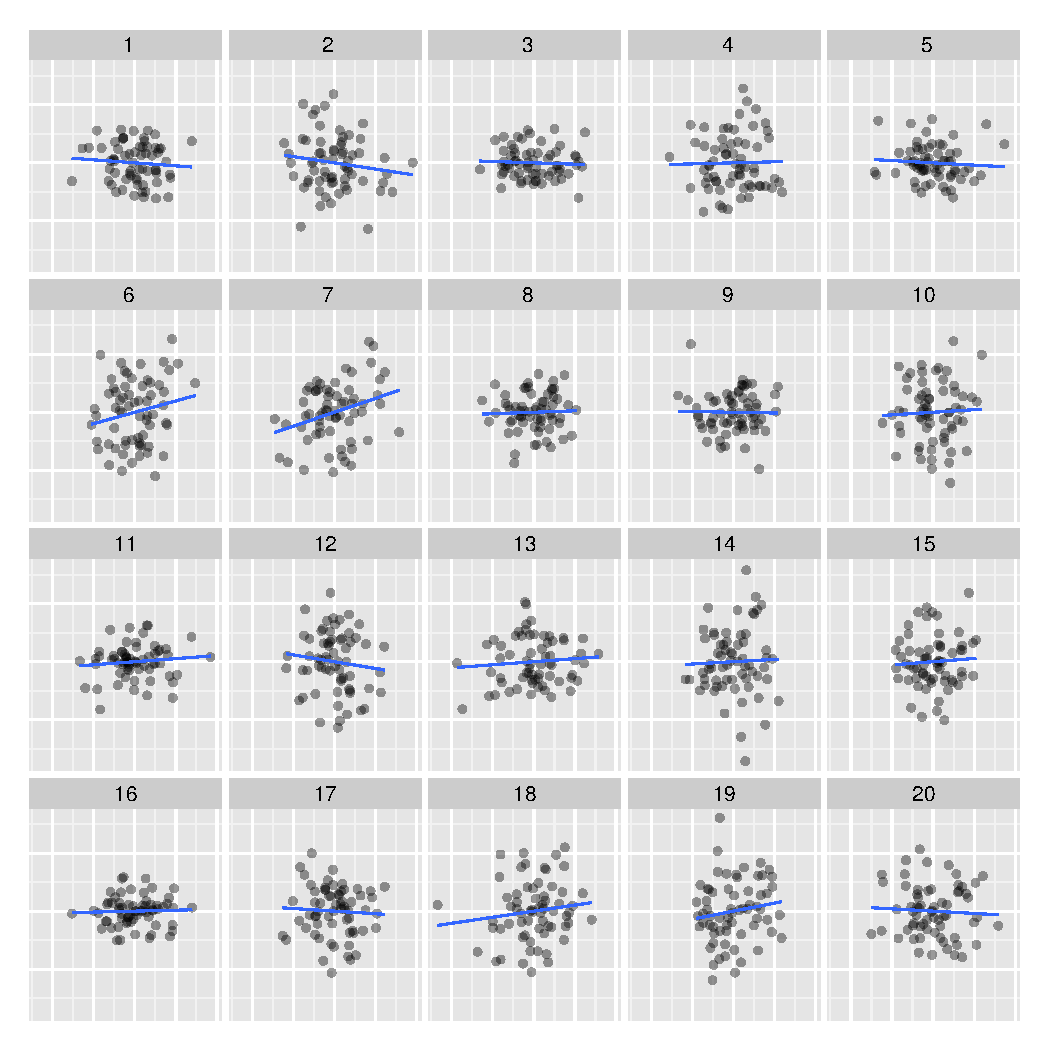
\includegraphics[width=\textwidth]{normexam_uncorr_lineup13.pdf}
%	\caption{\label{fig:ranef-uncorr}  Lineup testing the need to allow for correlation between the two random effects. These 20 plots compare the predicted random intercept and slope for the model fit to the Exam data. Which is the real plot?}
%\end{figure}

%\paragraph{Comparing non-nested models.}
%If two non-nested models are being considered, visual inference can be used to investigate the goodness-of-fit of each model (see Section~\ref{sec:checking} for further discussion). If inadequacies are discovered in one model but not in the other, then this support the use of the properly specified model. This approach is similar in concept to comparing the AIC from each model; however, by focusing on an investigation of how the true data depart from the assumptions made by the model we can see why one may be preferred.


%------------------------------------------------------------------------------------
\section{Model checking}\label{sec:checking}
%------------------------------------------------------------------------------------

In the formulation of model \eqref{eq:hlm} we make a number of assumptions that must be satisfied. In this section we discuss how residual plots can be used with lineups to check the assumptions of homogeneous residual variance, linearity, and normality of the random effects. While we only focus on these assumptions, the discussion is general enough to reveal how visual inference could be extended to check other aspects of the model.

%
%The lineup protocol presents a unified approach to overcome the difficulties encountered when checking the validity of a hierarchical linear model. The only change necessary to utilize this approach to model checking is the generation of null plots, for which we use the parametric bootstrap. Consequently, the ``standard'' residuals plots can be used within this framework in order to overcome the subjectiveness of interpretation and identification of artificial structures, making visual inference a natural extension of conventional model checking. In this section we discuss several examples of lineups that we have found useful for model checking; however, we do not intend to present an exhaustive overview.


\subsection{Homogeneity of variance}
%\subsubsection{Conventional practices}\label{sec:conv-check}
%------------------------------------------------------------------------------------

Model~\eqref{eq:hlm} assumes homogeneity of the within-group variance. To check this assumption must we verify the homogeneity of the within-group residual variance across the levels of all explanatory variables and check that the within-group variance is also constant across groups. Such investigations are often carried out using plots of the level-1 residuals; however, the interpretation of these plots is error prone.
For example, consider investigating the appropriateness of this assumption for the GSCEE data. 
%To check the homogeneity of variance across the values of the explanatory variables we utilize plots of the level-1 residuals.
%Such plots are appropriate to check the assumptions of linearity and homoscedasticity at each level of the model. 
%The lineup in 
Figure~\ref{fig:constvar1} shows a lineup of 20 plots of the level-1 residuals against (standardized LRT scores)$^3$, one of the explanatory variables included in the model. If any panel of this lineup is considered separately, an analyst may come to the conclusion that the within-group variance decreases as (standardized LRT scores)$^3$ increases; however, inserting the true plot into the lineup forces the analyst to consider the features such a plot will exhibit under the null hypothesis of homogenous variance. Based on the lineup, is there a violation of this model assumption? If we identify the true plot (panel $\sqrt{121} - 8$) this provides evidence of a violation, but if we are unable to, this provides evidence that any structure observed in the plot is artificial.

\al{A second example of this type of lineup is given in Figure~\ref{fig:constvar2}, which compares the level-1 residuals to pressure in the dialyzer study (see Section~\ref{data:dialyzer}). In this example XXX of XXX observers identified the true plot (panel $2^3 - 5$), providing evidence of heteroscedasticity. Comparing the two lineups reveals that the patterns that can be expected in any given residual plot differ depending on the data set. The use of lineups incorporates the comparison of the data to what is expected, eliminating the subjective interpretations we encounter with the use of single plots. }

\begin{figure}
	\centering
	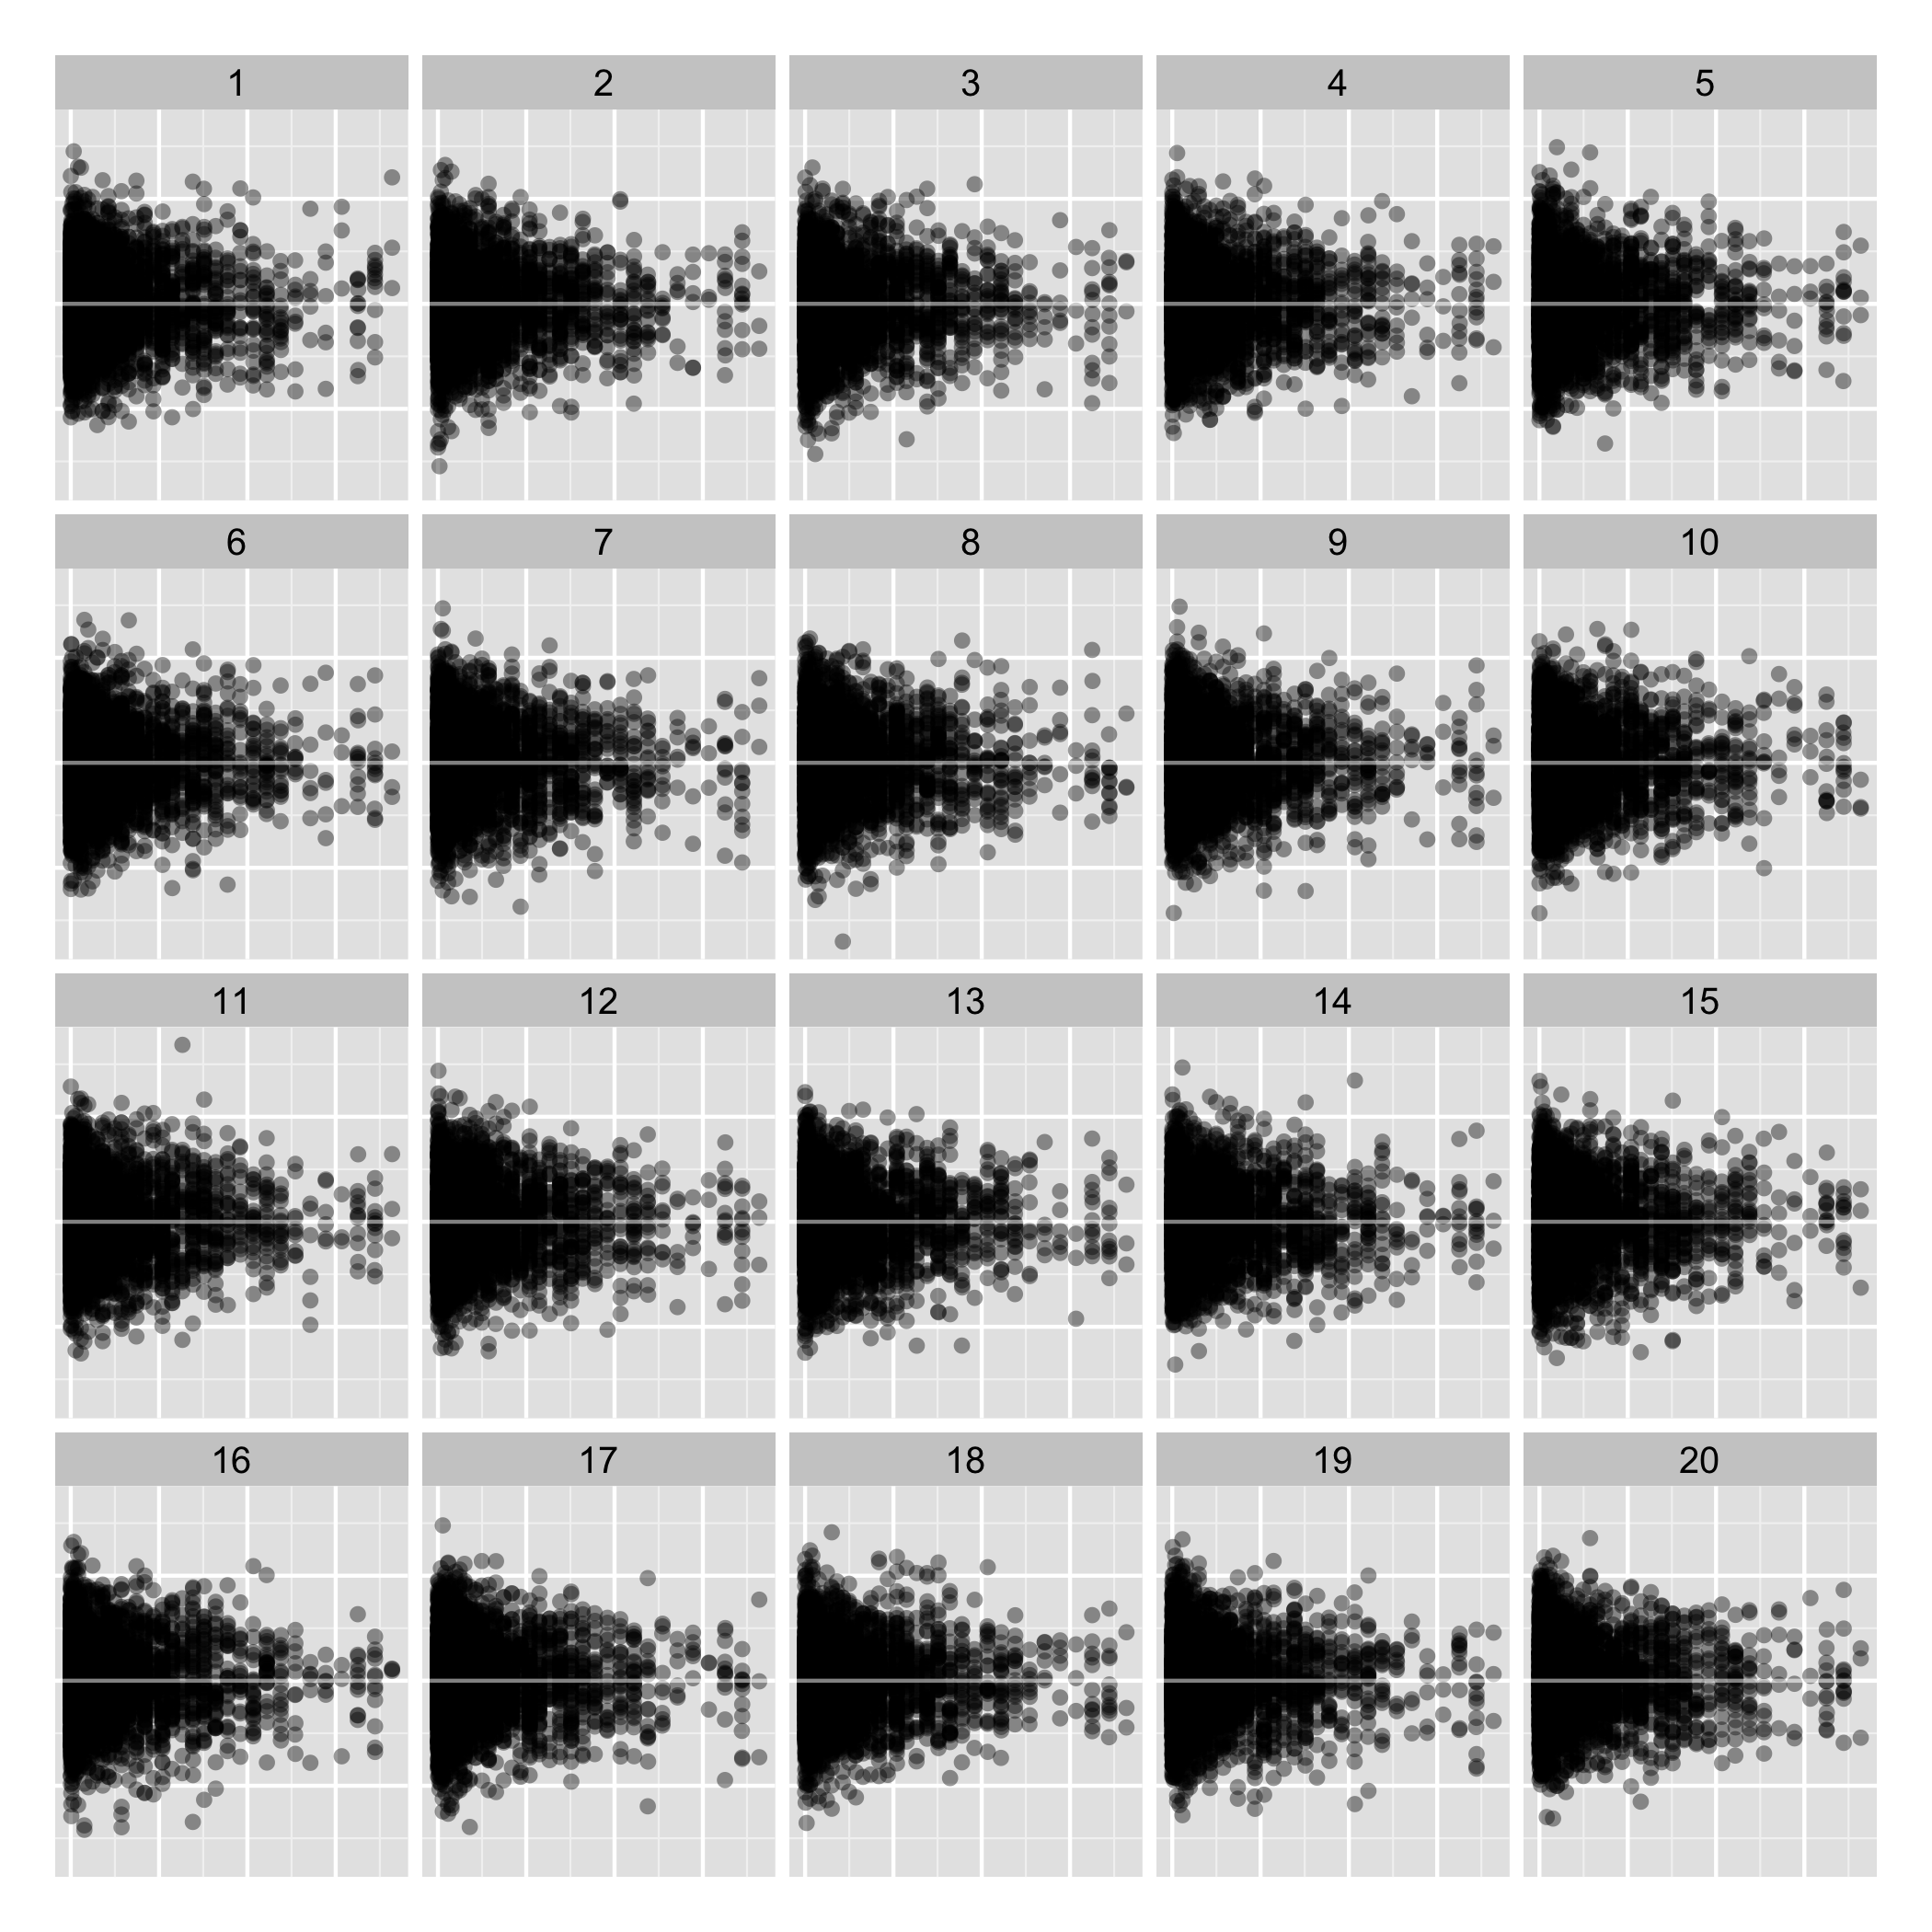
\includegraphics[width=\textwidth]{normexam_constvar_lineup3.png}
	\caption{\label{fig:constvar1} 
	Lineup testing homogeneity of the level-1 residuals. Which of the plots is the most different? Which feature led you to your choice?}
%	Lineup of 20 scatterplots of level-1 residuals against (standardized LRT)$^3$ used to test the assumption of homogeneous level-1 residual variance.  Which is the real plot?}
\end{figure}

\begin{figure}
	\centering
	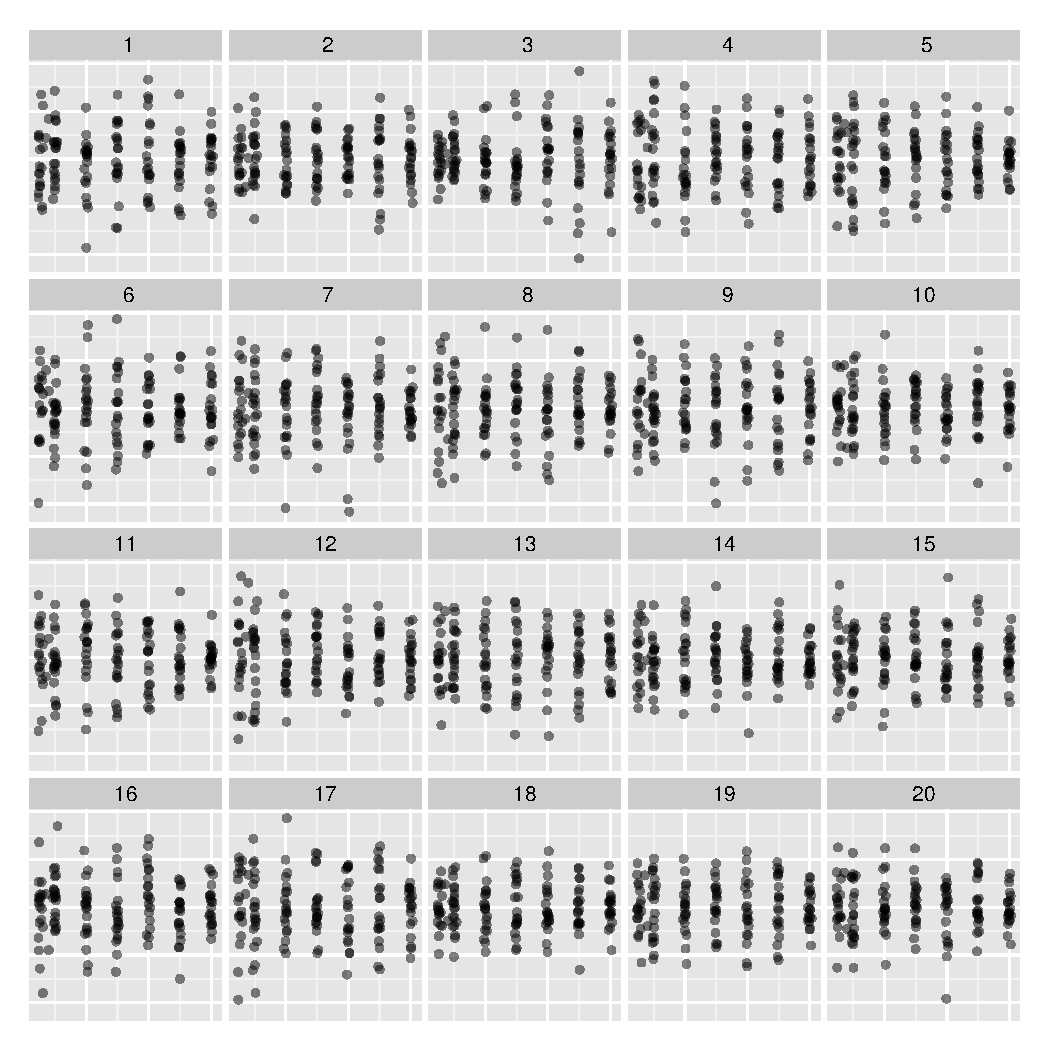
\includegraphics[width=\textwidth]{dialyzer-heterogeneous-lineup3.pdf}
	\caption{\label{fig:constvar2} 
	Lineup testing homogeneity of the level-1 residuals. Which of the plots is the most different? Which feature led you to your choice?}
%	Lineup of 20 scatterplots of level-1 residuals against pressure used to test the assumption of homogeneous level-1 residual variance for the dialyzer study.  Which is the real plot?}
\end{figure}

%\paragraph{Testing homoscedasticity across groups.}
Residual scatterplots are useful in checking that level-1 residuals are homoscedastic, but they do not investigate potential differences in variability across groups. To visualize this assumption, we suggest using side-by-side boxplots of the level-1 residuals. When the plots are considered individually, unbalanced group sizes will cause artificial structure in these plots. 
%This is to be expected as the variance of the sampling distribution of the level-1 residuals within each group, $\var \left( s_i^2 \right) = \left(2 \left( \sigma_i^2 \right)^2 \right) \big/ (n_i - r_i)$, where $r_i = \mathrm{rank}(\bm{X}_i)$, depends on the group size, $n_i$.
To overcome this difficulty, we create a lineup of side-by-side boxplots for each group ordered by their interquartile range (IQR), which we have come to call a ``cyclone'' plot. Figure~\ref{fig:badcyclone} shows a lineup of cyclone plots for 66 patients in a longitudinal study investigating the ability of Methylprednisolone to treat patients with severe alcoholic hepatitis (see Section~\ref{data:ahd} for details). The true plot (panel $2^3-4$) is easily identified from the field of null plots \al{(by XXX of XXX observers)} revealing heteroscedasticity across groups that cannot be detected by other residual plots. 


\begin{figure}
	\centering
	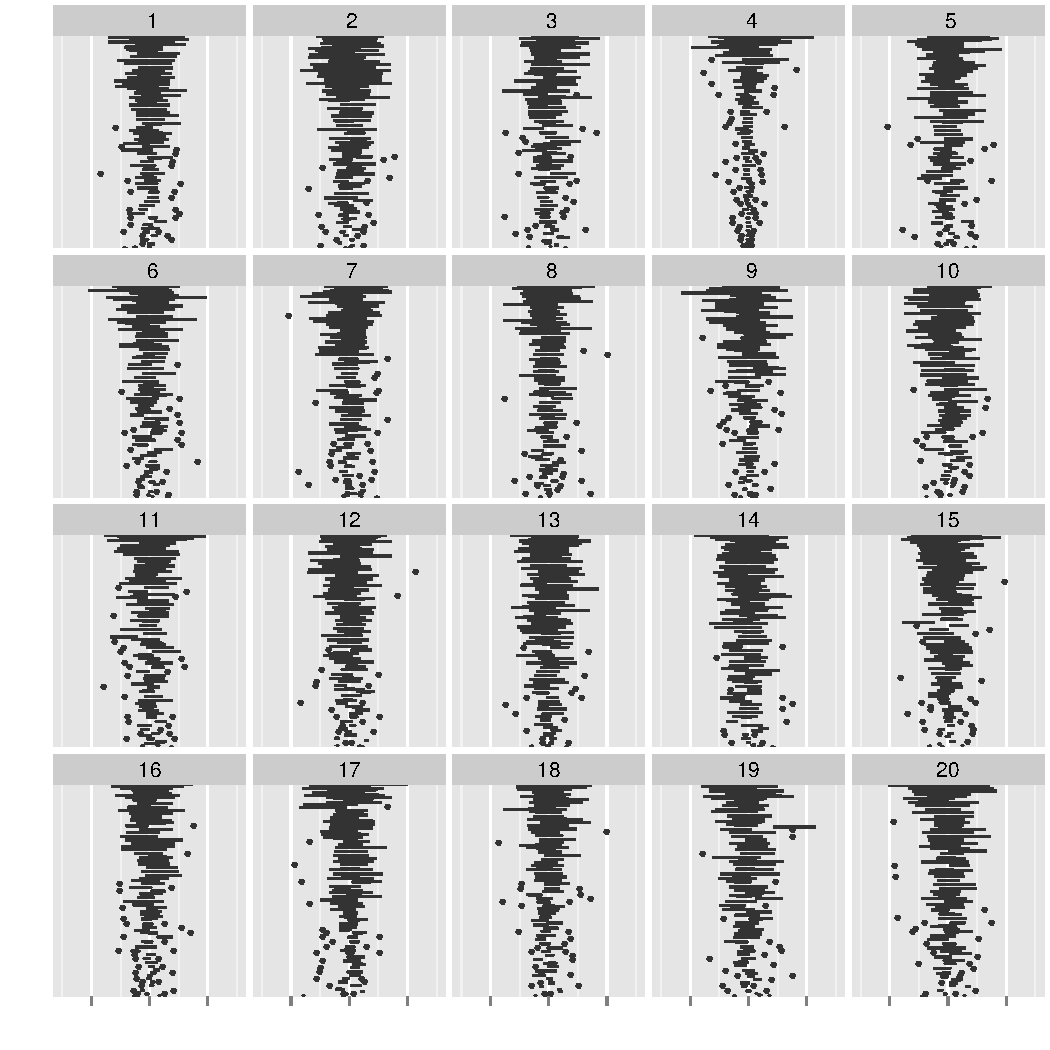
\includegraphics[width=\textwidth]{ahd_badcyclone4.pdf}
	\caption{\label{fig:badcyclone} 
	Lineup testing homogeneity of the level-1 residuals between groups. Which of the plots is the most different? Which feature led you to your choice?}
%	Lineup of 20 boxplots (ordered by IQR) of level-1 residuals used to test the assumption of homogeneous level-1 residual variance.  Which is the real plot?}
\end{figure}

An alternative approach to detect homoscedasticity of the level-1 residuals across groups is to use a \al{test based on the} standardized measure of dispersion given by
%
\begin{equation}\label{eq:d}
	d_i = \frac{\log\left( s_i^2 \right) - \left[ \sum_i (n_i - r_i) \log\left( s_i^2 \right) / \sum_i  (n_i - r_i) \right]}{\left(2 / (n_i - r_i)\right)^{1/2}}
\end{equation}
%
where $s_i^2$ is the residual variance within each group based on separate ordinary least squares regressions  \citep{Raudenbush:2002}. The test statistic is then
%
\begin{equation}
	H = \sum_{i=1}^{g^*} d_i^2
\end{equation}
%
which has an approximate $\chi^2_{g^*-1}$ reference distribution when the data are normal and the group sizes are ``large enough''. Here we use $g^*$ because ``small'' groups may be excluded from the calculation as small group sizes provide less reliable information about the residual variance, but this is a subjective choice. A common rule of thumb is to exclude groups with samples sizes smaller than 10. If the distributional assumptions are violated, or we do not have large enough group sizes,  the approximation to the $\chi^2$ distribution breaks down. In the Methylprednisolone study each subject was observed at most 5 times, with 19 subjects dropping out of the study early. Due to the small group sizes the $\chi^2$ approximation is inappropriate, forcing the analyst to rely on simulation to construct the sampling distribution of the test statistic, which is computationally more demanding than the generation of 19 null plots.


%\begin{figure}
%	\centering
%	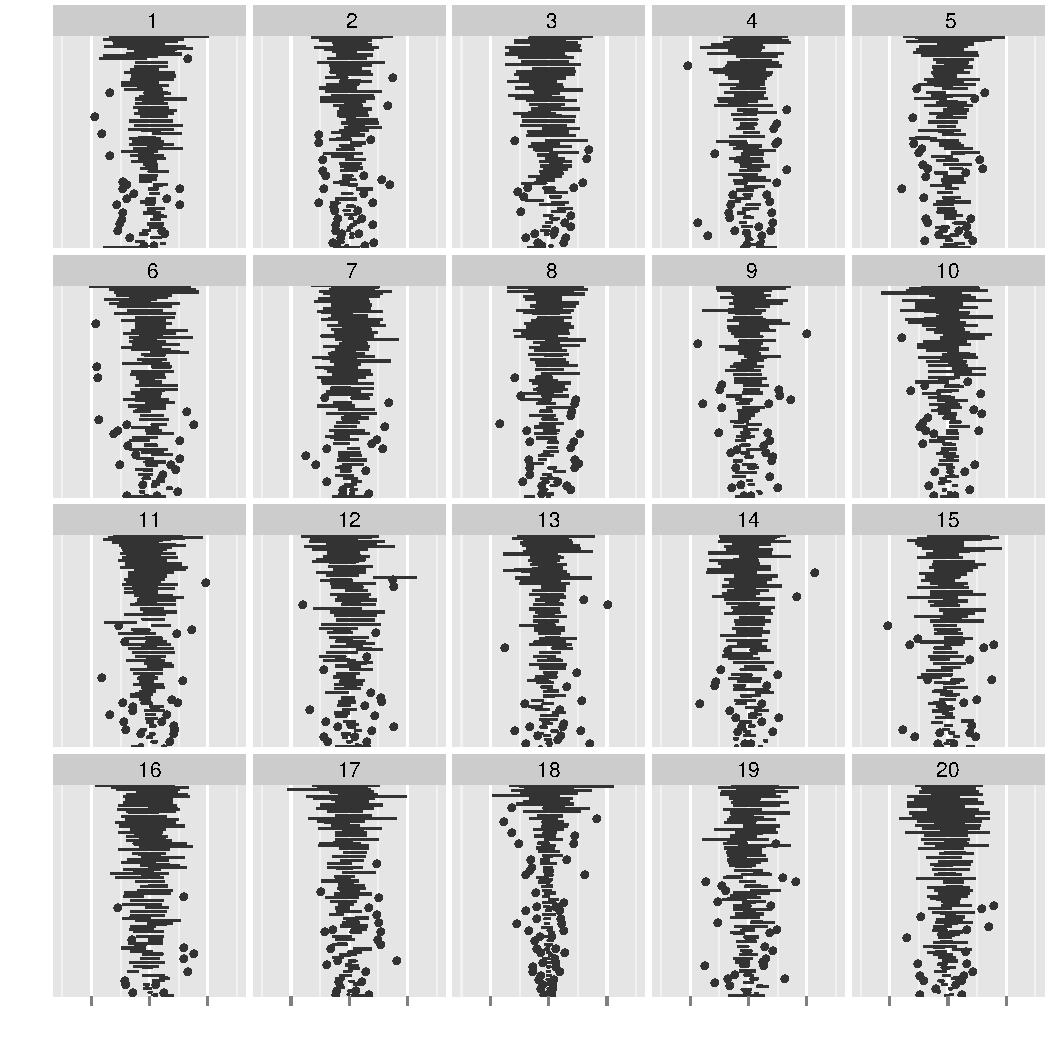
\includegraphics[width=\textwidth]{ahd_badcyclone5.pdf}
%	\caption{\label{fig:badcyclone} Lineup of 20 boxplots (ordered by IQR) of level-1 residuals used to test the assumption of homogeneous level-1 residual variance.  Which is the real plot?}
%\end{figure}

%\begin{figure}
%	\centering
%	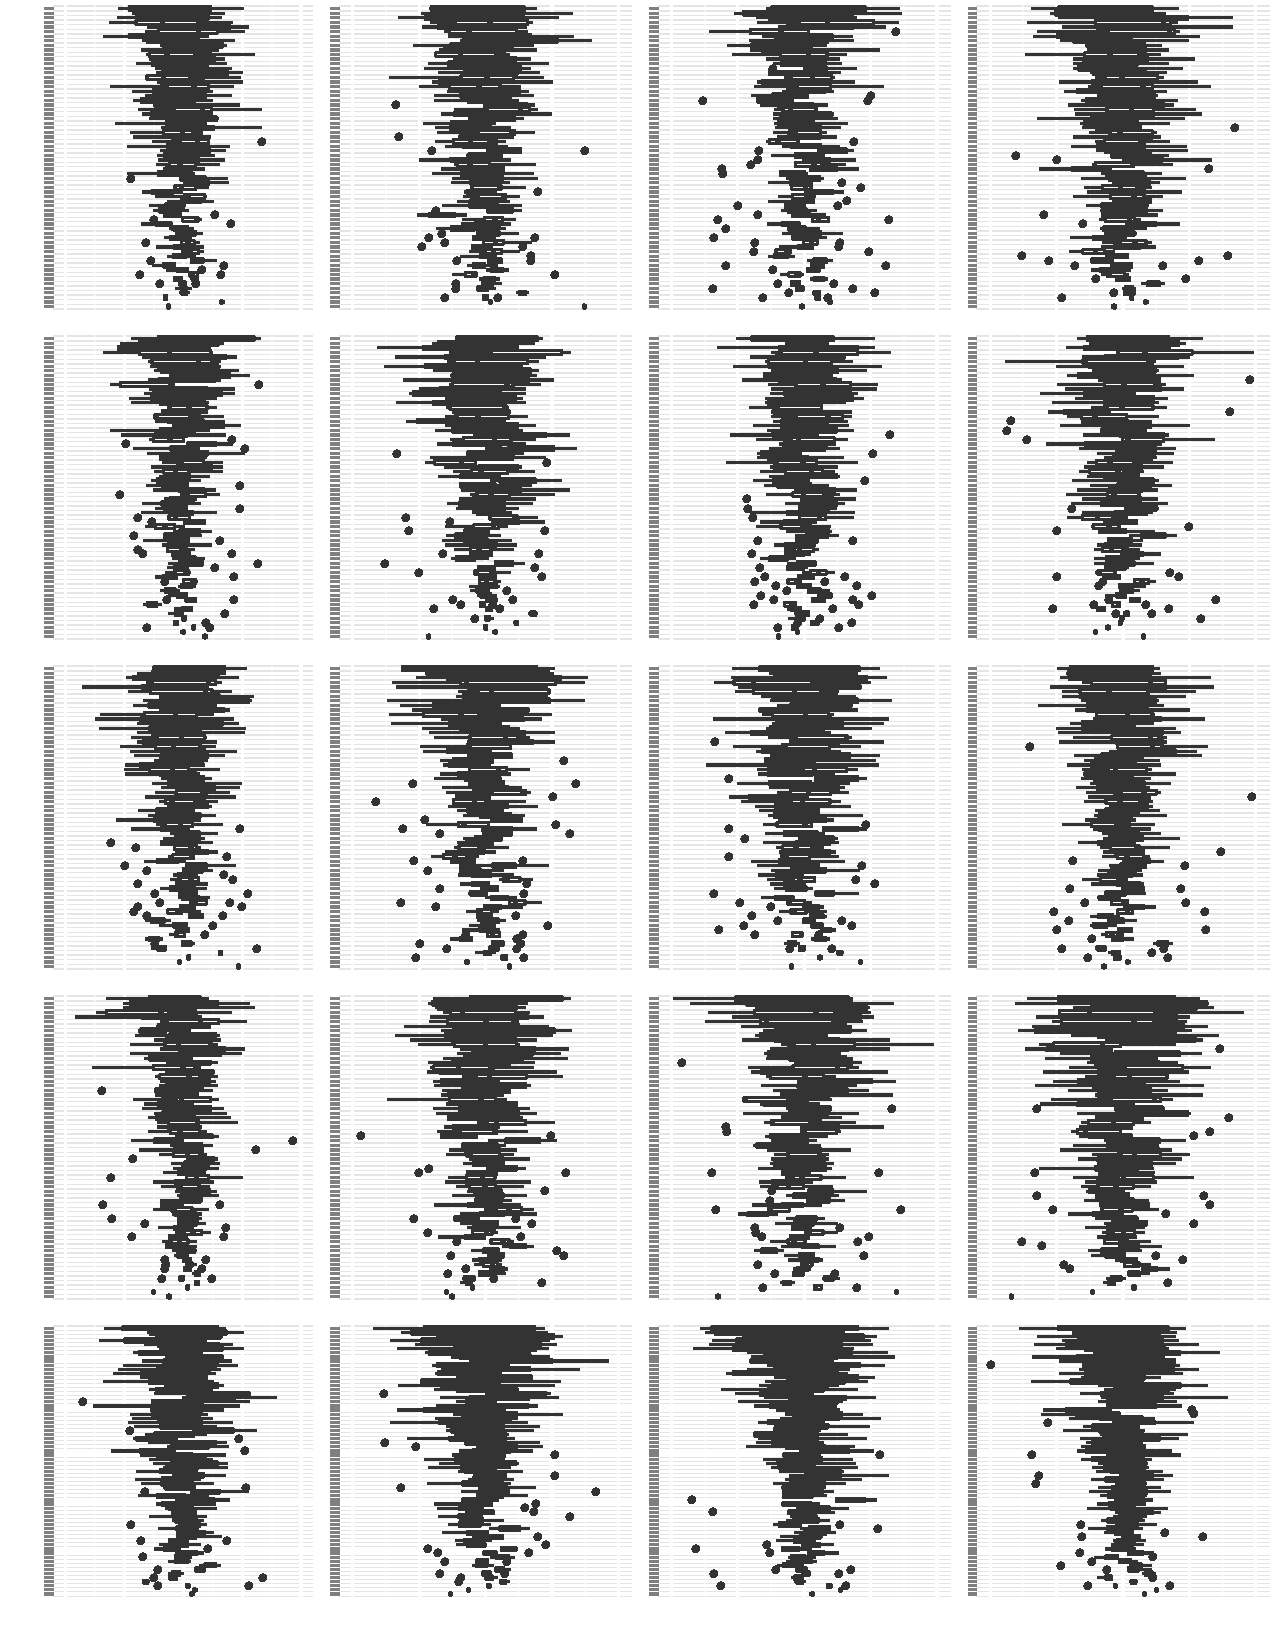
\includegraphics[width=\textwidth]{ahd_goodcyclone13.pdf}
%	\caption{\label{fig:goodcyclone} Lineup of 20 boxplots (ordered by IQR) of level-1 residuals used to test the assumption of homogeneous level-1 residual variance.  Which is the real plot?}
%\end{figure}


\subsection{Linearity}
%------------------------------------------------------------------------------------

\al{
Scatterplots with smoothers can also be used to check that the relationship between the explanatory variables and response variable is in fact linear. Figure~\ref{fig:linearity} shows such a lineup testing the linearity of an observation-level explanatory variable. Out of XXX observers, XXX identified the true plot (panel $2^4 + 1$), providing evidence that the mean structure is misspecified. This example comes from the dialyzer study and considers a model with only a linear and quadratic terms for transmembrane pressure. It is clear that a higher-order polynomial is required.

To extend checks of linearity to group-level variables we suggest the use of the level-2 residuals. Additionally, when categorical predictors are investigated, side-by-side boxplots should be used.
}


%To check the assumption of linearity we suggest the use of scatterplots with smoothers and boxplots of both the residuals (either level-1 or -2) against the fitted values of an explanatory variable. If the assumption of linearity is upheld, then the residuals plots will exhibit ``random scatter.'' 
%%As illustrated in the previous section, such plots are also useful in checking for homogeneity of variance, but in that situation different deviations from random scatter are of interest.
%\alnote{I will write more here.}

\begin{figure}
	\centering
	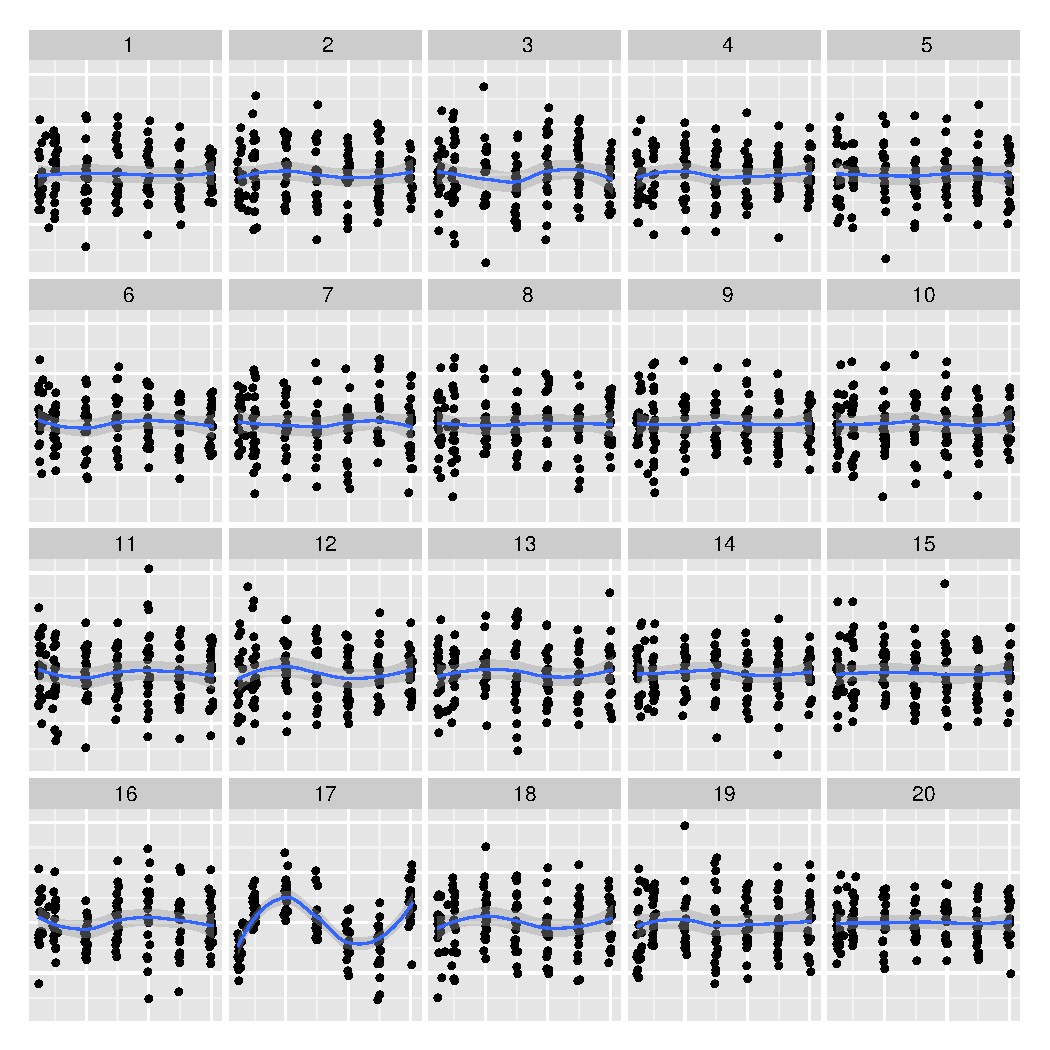
\includegraphics[width=\textwidth]{dialyzer-nonlinear-lineup17.pdf}
	\caption{\label{fig:linearity} Lineup testing testing for nonlinearity of a covariate. Which of the plots is the most different? Which feature led you to your choice?}
	%Lineup of 20 scatterplots of level-1 residuals against pressure with a LOESS smoother used to test the assumption of linearity for the dialyzer study.  Which is the real plot?}
\end{figure}

\subsection{Normality}
\hh{This section consists of two parts: we first discuss how to assess distributional assumptions in hierarchical models, which are complicated by confounding issues between levels of residual structures; in the second part we assess power of visual normality tests based on three different Q-Q plot designs.}
%------------------------------------------------------------------------------------

\subsubsection{Assessing normality of the random effects}
%------------------------------------------------------------------------------------

%Quantile-Quantile (Q-Q) plots \citep{Wilk:1968} are often used as an informal check of the distributional assumptions made on the level-1 and -2 residuals; however, an interrelationship between the residual quantities exists in hierarchical linear models that can render such an assessment inappropriate. 

\al{Recall that in model~\eqref{eq:hlm} we assume that the random effects, $\bm{b}_i$, are a random sample from $\mathcal{N}(\bm{0},\ \bm{D})$ and are independent from the error terms, $\bm{\varepsilon}_i$, which are assumed to be a random sample from $\mathcal{N}(\bm{0},\ \sigma^2 \bm{I}_i)$. In many situations, however, the predicted random effects are highly influenced (i.e., confounded) by the error terms. Consequently, traditional checks for normality such as Q-Q plots and the Anderson-Darling test are not appropriate. Formally this is seen by the}
strong assumptions that are required for the empirical distributions of the residuals in the linear mixed-effects models to converge in probability to their true distributions \citep[Theorem 3.2 and Lemma 3.1]{Jiang:1998vt}. If these assumptions are not satisfied, then the empirical distribution of the residuals may not resemble the hypothesized distribution under a properly specified model. When this occurs individual Q-Q plots will often lead to erroneous conclusions about the distributional assumptions which can be overcome, at least partially, using lineups.

Figures~\ref{fig:qqlineup-1} and \ref{fig:qqlineup-t} illustrate the use of lineups to test the distributional assumptions in a hiearachical linear model. Figure~\ref{fig:qqlineup-1} presents a lineup of the predicted random slopes from the radon study (see Section~\ref{data:radon} for details), in which group sizes are very unbalanced and there is a high degree of shrinkage.
%Both lineups present simulated Q-Q plots of predicted random effects following the design of the radon study (see Section~\ref{data:radon} for details), in which group sizes are very unbalanced and there is a high degree of shrinkage. 
Confidence bands based on the normal distribution were applied to each lineup and reveal that the empirical distribution of the predicted random effects---both for the null plots and true plots---does not align with a normal distribution. While such confidence bands show the relationship of the predicted random effects to the hypothesized distribution, it is known that this is an ill conceived comparison in many cases; however, the lineups are not comparing the predicted random effects to the normal distribution, but rather are comparing the empirical distribution of the random effects between the null and observed plots. Consequently, the conclusions drawn from the lineups relate to evidence of consistency between the true plot and what is expected under a properly specified model. For example, the true plot in Figure~\ref{fig:qqlineup-1} (panel $2^4 - 6$) is indistinguishable from the null plots \al{(none of 23 observers identified this plot)}, providing no evidence of a violation of normality; however, when compared only to the normal distribution, the observed Q-Q plot would %, \al{in our opinion}, 
be \hh{rejected by any standard test for normality} \al{(e.g., the $p$-value of the Anderson-Darling test is .0004 for the panel of the data).} 
\hh{Panel \#5 was identified  most often from the lineup in Figure~\ref{fig:qqlineup-1}; it was picked by 13 out of 23 observers. All other panels were selected at most two times. }
Additionally, this example shows that even the null plots that were generated from a normal distribution no longer look normal after after model estimation---in fact, 16 of the null plots fail the Anderson-Darling test of normality at a significance level of .05
% \hh{All of the other panels are created from samples from a normal distribution, but after the model fit, they} \al{no longer} \hh{look normal---in fact, 16 of them fail the Anderson-Darling test of normality at a significance level of .05.}

% In Figure~\ref{fig:qqlineup-t} we can identify the true plot (panel $\sqrt{49} - 1$) providing evidence that the assumption of normality is violated, which is in fact the case as the true plot was constructed from random effects simulated from a $t_3$ distribution. 
To determine whether lineups can detect distributional violations we constructed another lineup where the ``true plot'' was constructed from random effects simulated from a $t_3$ distrubution. This lineup is show in Figure~\ref{fig:qqlineup-t}. \al{XXX out of XXX} identified the true plot (panel $\sqrt{49} + 3$), providing evidence against the null hypothesis of normality.  
 The fact that we can distinguish the true plot from the null plots in Figure~\ref{fig:qqlineup-t} indicates that lineups of Q-Q plots provide an avenue for distributional assessment where conventional methods fail. Further investigation is needed to explore limitations of this approach, as there are undoubtably situations where this approach will be unsuccessful, but this is outside the scope of the current paper.  The ability of a lineup to distinguish a $t$ distribution for the random effects in the radon study shows that the approach has fewer limitations than conventional approaches, justifying our preference.
%The utility of lineups in this case relies on whether the empirical distributions of predicted random effects are expected to be different under model violations, which was the case in this example. We add this as a 


\begin{figure}
	\centering
%	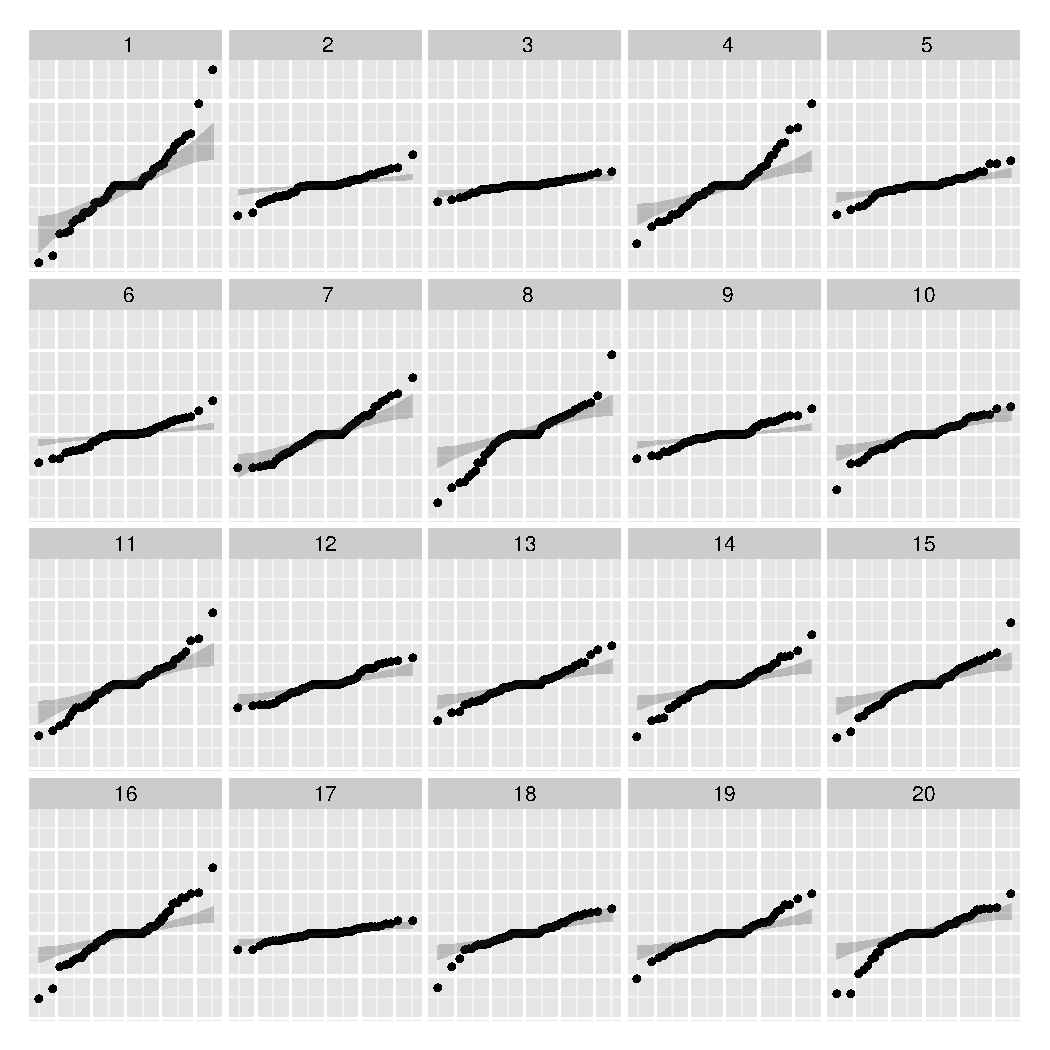
\includegraphics[width=\textwidth]{qqplot_normranef_slope_lineup11.pdf}
	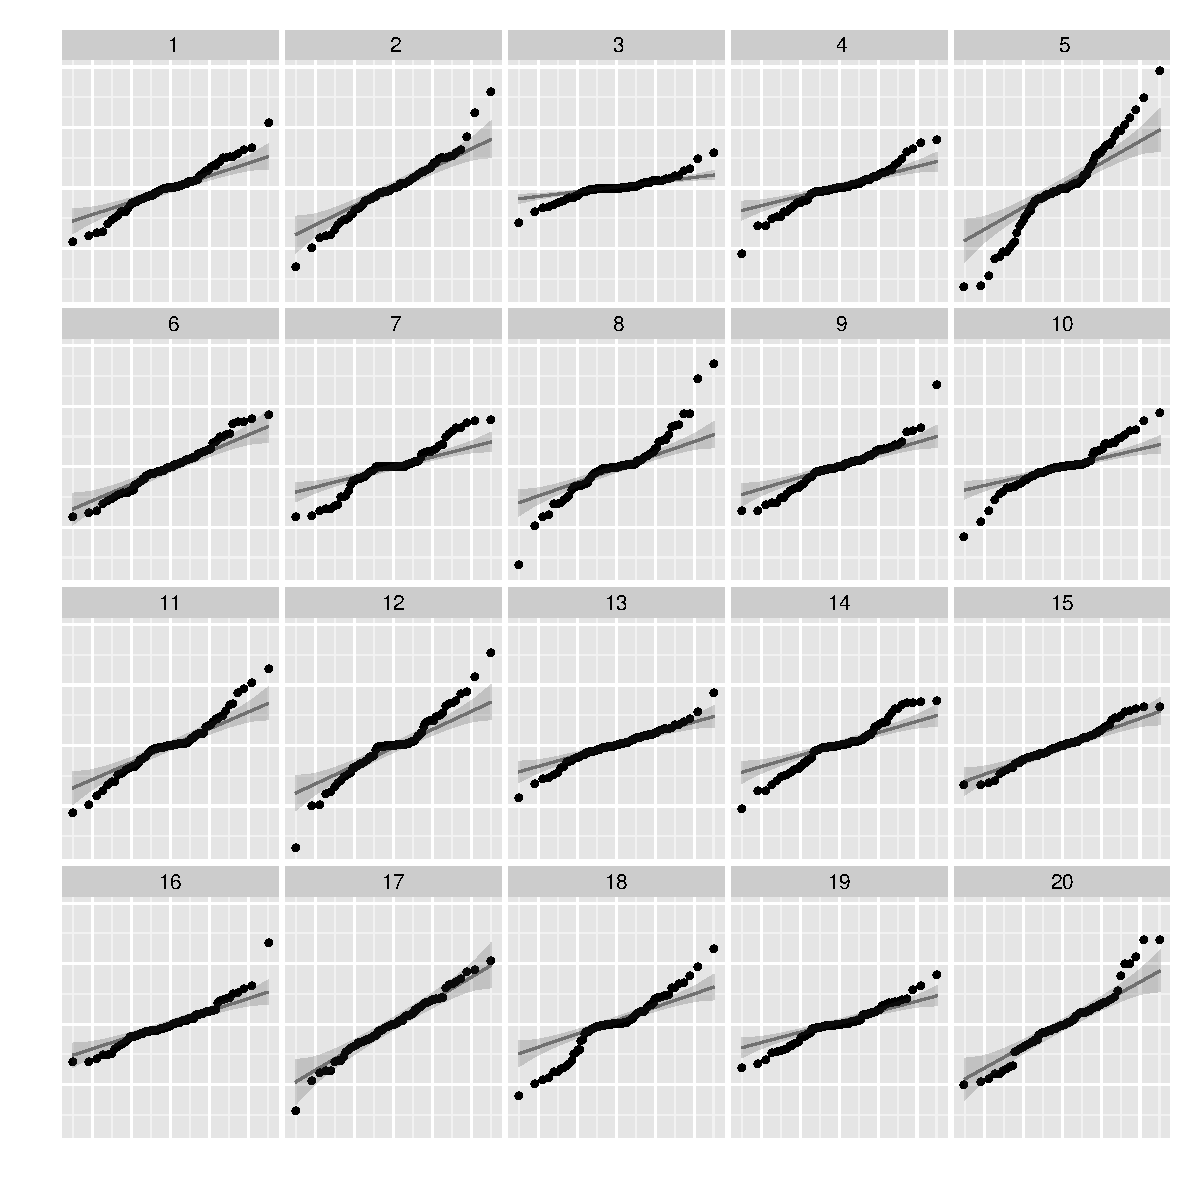
\includegraphics[width=\textwidth]{filebab6182c2e84}
	\caption{\label{fig:qqlineup-1}
	Lineup testing testing for normality of the random slope for the radon data. Which of the plots is the most different? Which feature led you to your choice?}
\end{figure}

\begin{figure}
	\centering
	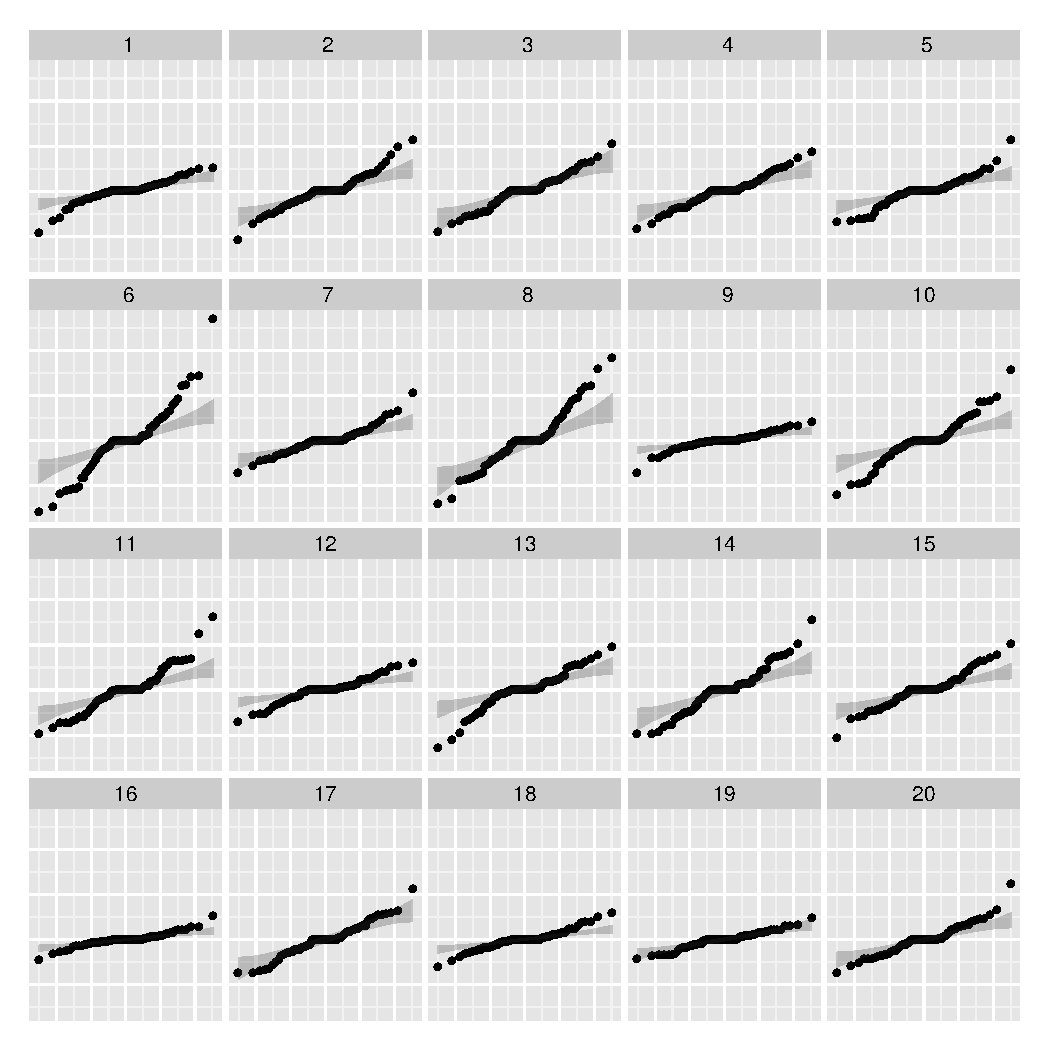
\includegraphics[width=\textwidth]{qqplot_tranef_slope_lineup6.pdf}
	\caption{\label{fig:qqlineup-t} Lineup testing testing for normality of the random slope for the radon data. Which of the plots is the most different? Which feature led you to your choice?}
\end{figure}



%\paragraph{Residual scatterplots/boxplots.} 
%One of the most common diagnostic plots is a scatterplot or boxplot of the residuals (either level-1 or -2) against the fitted values or an explanatory variable. Such plots are often used to check linearity of the variables included in the model and homoscedasticity of the level-1 residuals. Patterns in these plots indicate departures from the model assumptions, however, we have found that patterns seem to be detectable in properly specified models more often than in the classical linear model. This problem is more commonly seen in scatterplots. 

%\paragraph{Testing homoscedasticity across groups.}
%Residual scatterplots are often used to check the assumption of homoscedastic level-1 residuals, but such plots do no account for the potential differences in variability across groups. Side-by-side boxplots of the level-1 residuals can be used to visualize this assumption; however, unbalanced group sizes can cause artificial structure in such plots. This can be seen by considering the sampling distribution of the level-1 residual variance, which has variance $\var \left( s_i^2 \right) = \left(2 \left( \sigma_i^2 \right)^2 \right) \big/ (n_i - p_i)$ which depends on the group size. Alternatively, \cite{Raudenbush:2002} propose using a standardized measure of dispersion given by
%%
%\begin{equation}\label{eq:d}
%	d_i = \frac{\log\left( s_i^2 \right) - \left[ \sum_i (n_i - r_i) \log\left( s_i^2 \right) / \sum_i  (n_i - r_i) \right]}{\left(2 / (n_i - r_i)\right)^{1/2}}
%\end{equation}
%%
%where $s_i^2$ is the residual variance within each group and $r_i = \mathrm{rank}(\bm{X}_i)$. The test statistic is then
%%
%\begin{equation}
%	H = \sum_{i=1}^{m^*} d_i^2
%\end{equation}
%%
%which has an approximate $\chi^2_{m^*-1}$ reference distribution when the data are normal and the group sizes are ``large enough''. Here we use $m^*$ because ``small'' groups may be excluded from the calculation as small group sizes provide less reliable information about the residual variance, but this is a subjective choice. If the distributional assumptions are violated or we do not have large enough group sizes, then the approximation to the $\chi^2$ distribution breaks down.


%\paragraph{Quantile-Quantile plots.}
%Quantile-Quantile (Q-Q) plots are often used as an informal check of the distributional assumptions made on the level-1 and -2 residuals; however, an interrelationship between the residual quantities exists in hierarchical linear models that can render such an assessment inappropriate. Additionally, strong assumptions are required for the empirical distributions of the residuals in the hierarchical linear model to converge in probability to their true distributions \citep[Theorem 3.2 and Lemma 3.1]{Jiang:1998vt}. If these assumptions are not satisfied, then the empirical distribution of the residuals may not resemble the hypothesized distribution under a properly specified model. Consequently, Q-Q plots will often lead to erroneous conclusions about the distributional assumptions.


%\subsubsection{Proposals for visual inference}
%------------------------------------------------------------------------------------

%The lineup protocol presents a unified approach to overcome the difficulties encountered when checking the validity of a hierarchical linear model. The only change necessary to utilize this approach to model checking is the generation of null plots, for which we use the parametric bootstrap. Consequently, the ``standard'' residuals plots can be used within this framework in order to overcome the subjectiveness of interpretation and identification of artificial structures, making visual inference a natural extension of conventional model checking. In this section we discuss several examples of lineups that we have found useful for model checking; however, we do not intend to present an exhaustive overview.

%First we consider investigating the appropriateness of a hierarchical linear model based on plots of residuals against explanatory variables. Such plots are appropriate to check the assumptions of linearity and homoscedasticity at each level of the model. The lineup in Figure~\ref{fig:constvar1} was chosen to test the homoscedasticity of the level-1 residual variance across levels of (standardized LRT scores)$^3$. Here, the true plot (panel $2^3-3$) is indistinguishable from the null plots indicating that there is no evidence that the level-1 residual variance is non-constant across the values of (standardized LRT scores)$^3$. While this conclusion is apparent from the lineup, we believe this is not the case if the true plot is considered separately. In this case, an analyst might believe that the level-1 residual variance decreases as (standardized LRT scores)$^3$ increases, which, based on the lineup, is simply artificial structure. 
% 
%\begin{figure}
%	\centering
%	\includegraphics[width=\textwidth]{normexam_constvar_lineup5.pdf}
%	\caption{\label{fig:constvar1} Lineup of 20 scatterplots of level-1 residuals against (standardized LRT)$^3$ used to test the assumption of homogeneous level-1 residual variance.  Which is the real plot?}
%\end{figure}
%
%While lineups such as Figure~\ref{fig:constvar1} address the assumption of homogeneous level-1 residual variance, they do not speak to the assumption of homogeneous level-1 residual variance across all groups. To do this we propose using a lineup of boxplots for each group ordered by their interquartile range (IQR), which we have come to call a ``cyclone'' plot. Figure~\ref{fig:badcyclone} shows a lineup of cyclone plots for 66 patients in a longitudinal study investigating the ability of Methylprednisolone to treat patients with severe alcoholic hepatitis (see Section~\ref{data:ahd} for details). The true plot (panel $2^3-3$) is easily identified from the field of null plots revealing heteroscedasticity across groups that was not detected by other plots. In this longitudinal study each subject was observed at most 5 times, with 19 subjects dropping out of the study early. Due to the small group sizes, the $\chi^2$ approximation used by the numeric approach suggested by \cite{Raudenbush:2002} is inappropriate, so conventional testing would be forced to rely on simulation, which is computationally more demanding than the generation of 19 null plots.
%
%
%\begin{figure}
%	\centering
%	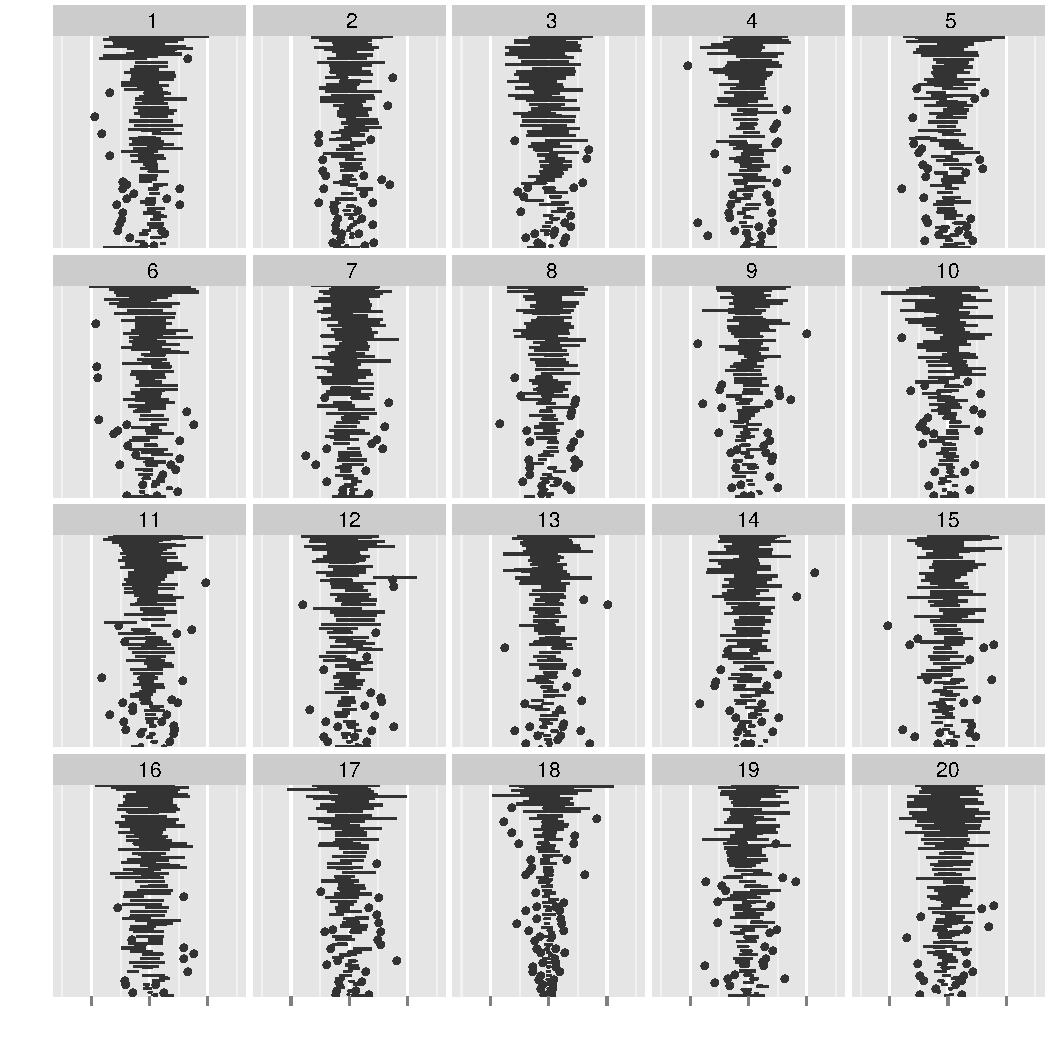
\includegraphics[width=\textwidth]{ahd_badcyclone5.pdf}
%	\caption{\label{fig:badcyclone} Lineup of 20 boxplots (ordered by IQR) of level-1 residuals used to test the assumption of homogeneous level-1 residual variance.  Which is the real plot?}
%\end{figure}
%
%\begin{figure}
%	\centering
%	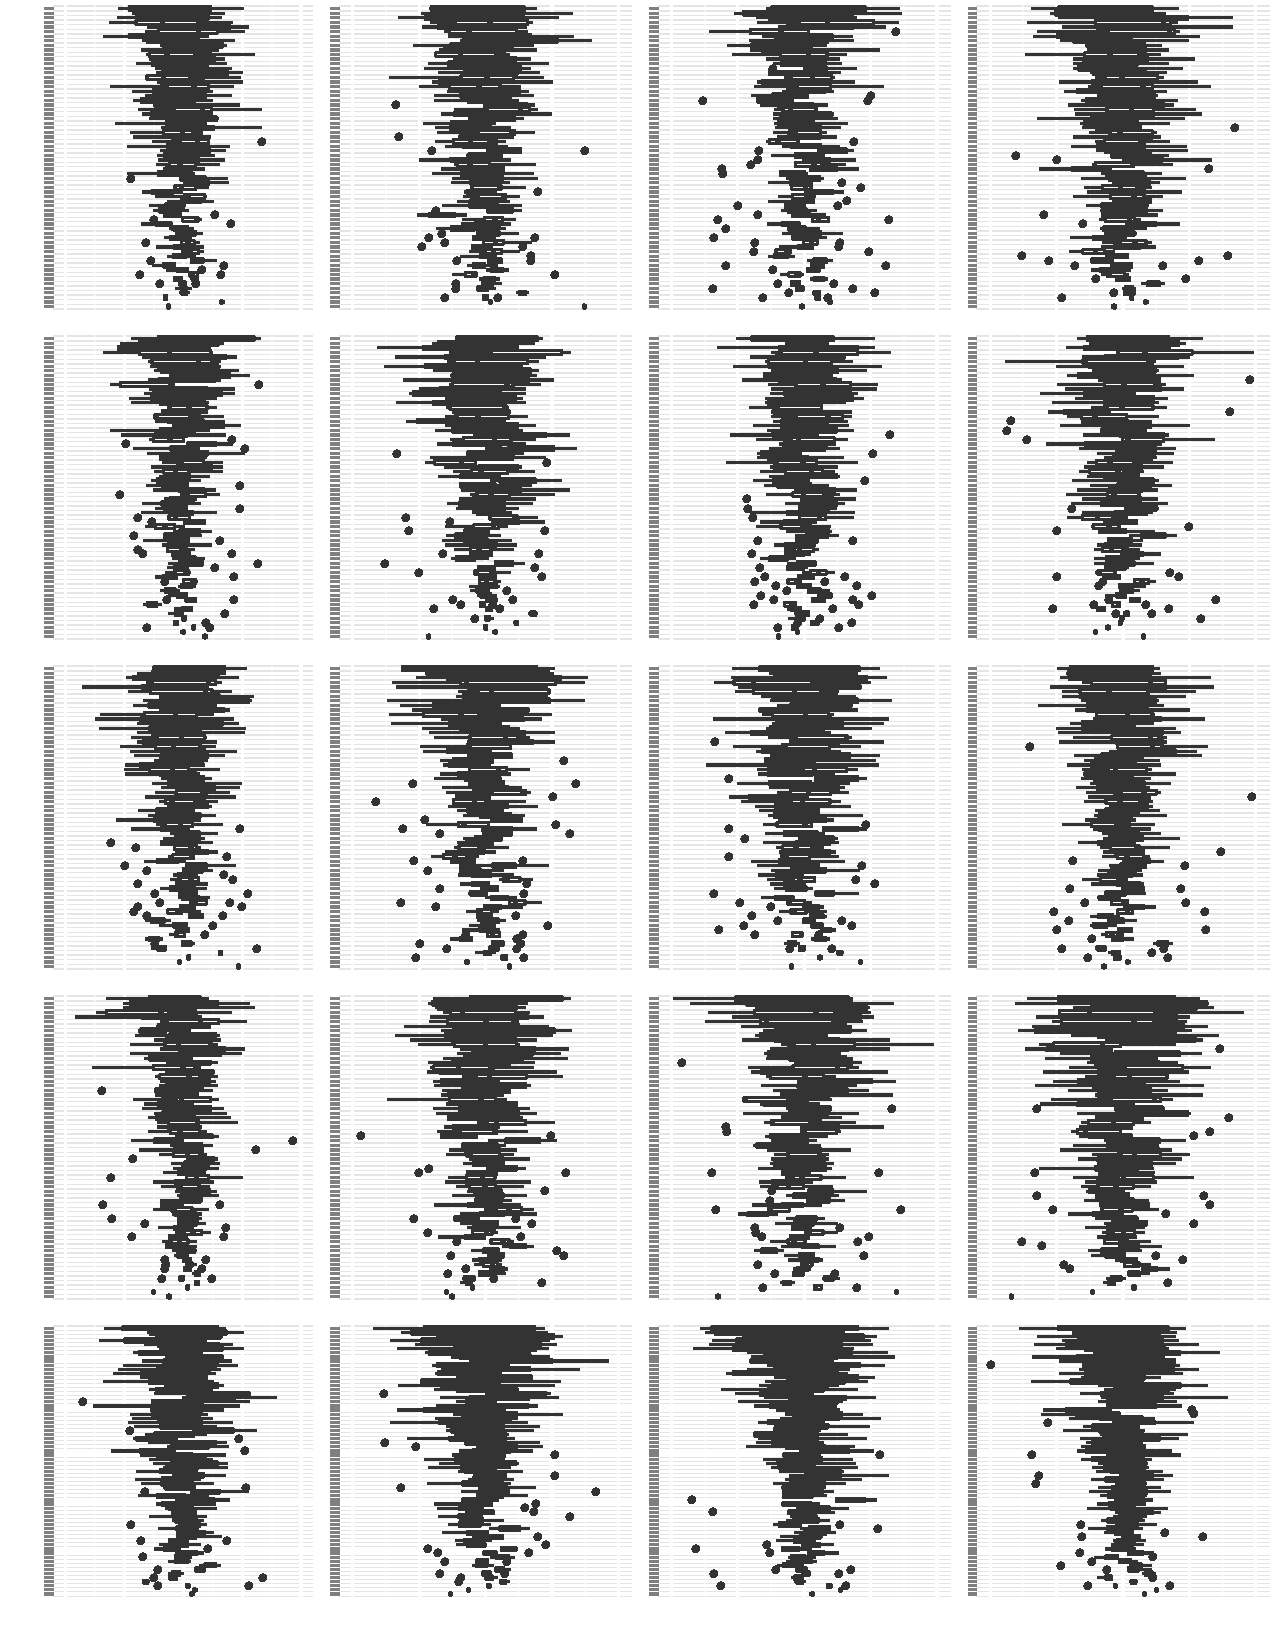
\includegraphics[width=\textwidth]{ahd_goodcyclone13.pdf}
%	\caption{\label{fig:goodcyclone} Lineup of 20 boxplots (ordered by IQR) of level-1 residuals used to test the assumption of homogeneous level-1 residual variance.  Which is the real plot?}
%\end{figure}


%Finally, the lineups presented in Figures~\ref{fig:qqlineup-norm} and \ref{fig:qqlineup-t} illustrate the use of lineups to test the distributional assumptions in a hiearachical linear model. Both lineups present simulated Q-Q plots of predicted random effects following the design of the radon study (see Section~\ref{data:radon} for details), in which group sizes were very unbalanced and there was a high degree of shrinkage. Confidence bands based on the normal distribution were applied to each lineup and reveal that the empirical distribution of the predicted random effects---both for the null plots and true plots---does not align with a normal distribution. While such confidence bands show the relationship of the predicted random effects to the hypothesized distribution, it is known that this is an ill conceived comparison in many cases; however, the lineups are not comparing the predicted random effects the normal distribution, but rather are comparing the empirical distribution of the random effects between null and observed plots. Consequently, the conclusions drawn from the lineups relate to evidence of consistency between the true plot and what is expected under a properly specified model. For example, the true plot in Figure~\ref{fig:qqlineup-norm} (panel $2^5 - 5$) is indistinguishable from the null plots, indicating no evidence of a violation of normality, but compared only to the normal distribution in a single Q-Q plot would be identified as a violation. In Figure~\ref{fig:qqlineup-t} we can identify the true plot (panel $\sqrt{49} - 1$) providing evidence that the assumption of normality is violated, which is in fact the case as the true plot was constructed from random effects simulated from a $t_3$ distribution. The fact that we can distinguish the true plot from the null plots in Figure~\ref{fig:qqlineup-t} indicates that lineups of Q-Q plots provide an avenue for distributional assessment where conventional methods fail. Further investigation is needed to explore limitations of this approach, as there are undoubtably situations where this approach will be unsuccessful, however, this is outside the scope of this paper.  The ability of a lineup to distinguish a $t$ distribution for the random effects in the radon study shows that the approach has fewer limitations than conventional approaches, justifying our preference.
%%The utility of lineups in this case relies on whether the empirical distributions of predicted random effects are expected to be different under model violations, which was the case in this example. We add this as a 
%
%
%\begin{figure}
%	\centering
%	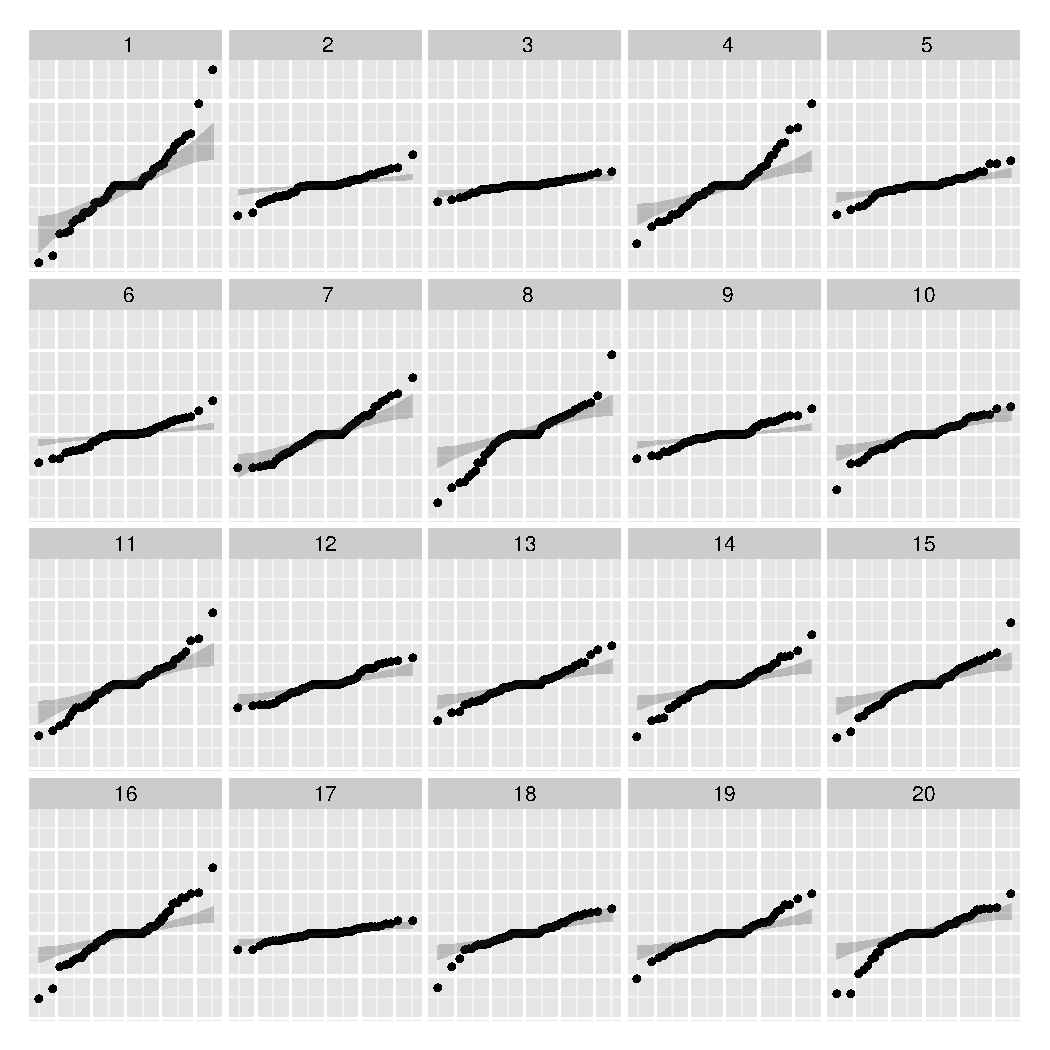
\includegraphics[width=\textwidth]{qqplot_normranef_slope_lineup11.pdf}
%	\caption{\label{fig:qqlineup-norm} Lineup of 20 normal Q-Q plots for the predicted random slope.  Which is the real plot?}
%\end{figure}
%
%\begin{figure}
%	\centering
%	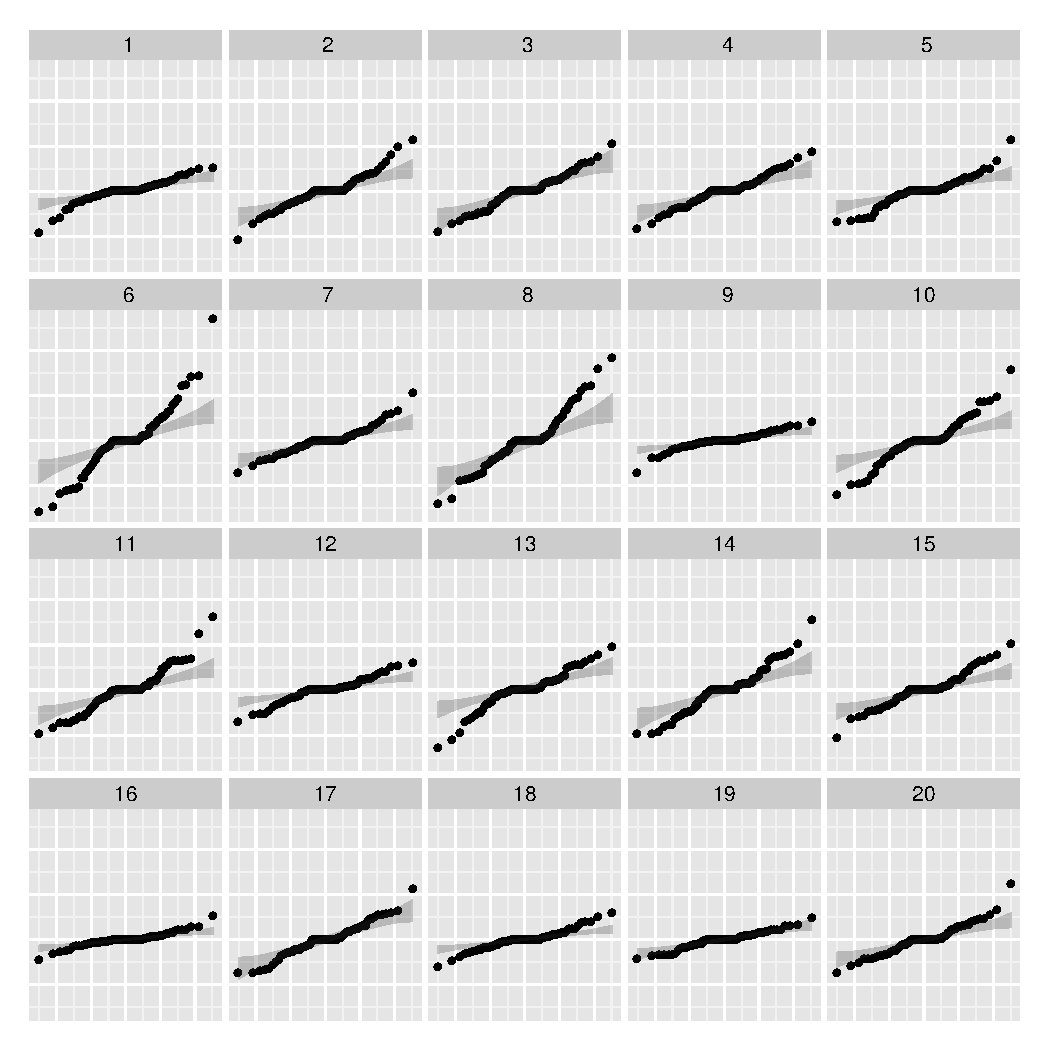
\includegraphics[width=\textwidth]{qqplot_tranef_slope_lineup6.pdf}
%	\caption{\label{fig:qqlineup-t} Lineup of 20 normal Q-Q plots for the predicted random slope.  Which is the real plot?}
%\end{figure}
%
%
%\todo[inline]{Should the below section headings be deleted?}
%
%%------------------------------------------------------------------------------------
%\section{Visual inference for hierarchical linear models}
%%------------------------------------------------------------------------------------
%
%In this section we discuss how visual inference can be implemented to conduct common tests for hierarchical linear models and to avoid misinterpreting residual plots. 
%
%
%\subsection{Model selection}
%%------------------------------------------------------------------------------------





%\begin{figure}
%	\centering
%	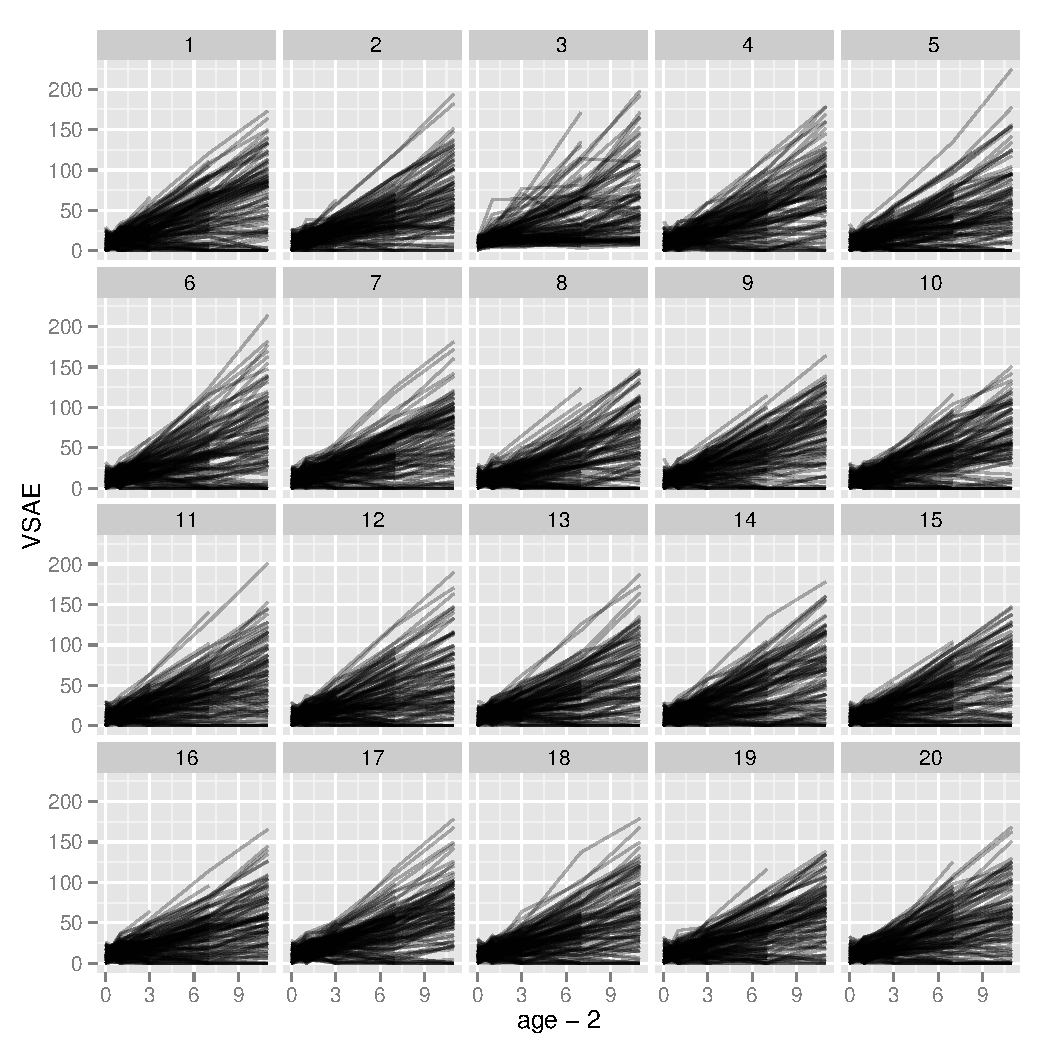
\includegraphics[width=\textwidth]{ranef1_lineup3.pdf}
%	\caption{\label{fig:lineup-ranef1} Lineup testing whether the random slope for $(\text{age} - 2)$ is sufficient, or if additional random effects are needed. These 20 plots display a child's VSAE trajectory. Which is the real plot?}
%\end{figure}
%
%\begin{figure}
%	\centering
%	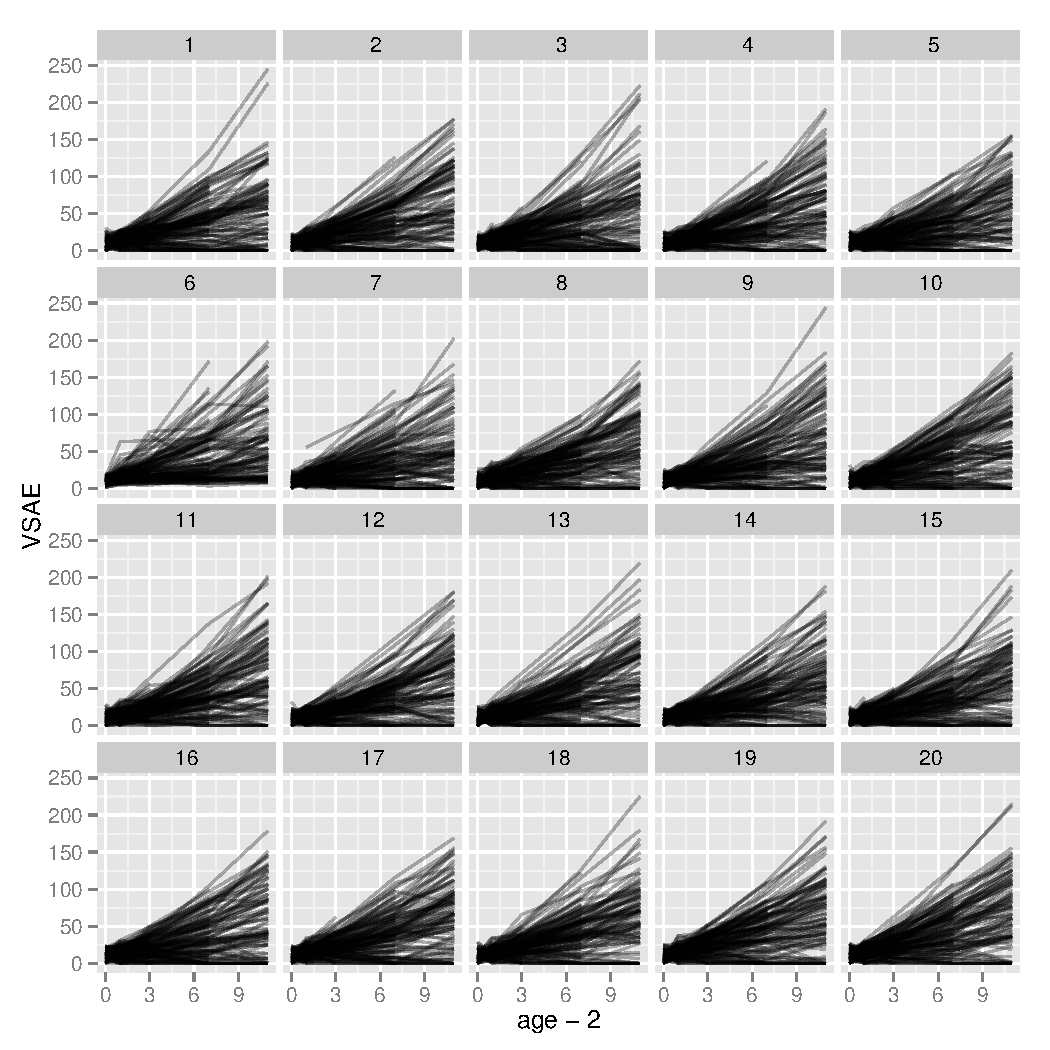
\includegraphics[width=\textwidth]{ranef2_lineup6.pdf}
%	\caption{\label{fig:lineup-ranef2} After adding a random effect for $(\text{age} - 2)^2$ we can construct the same lineup to see if we have a sufficient representation of the relationship between VSAE and age. These 20 plots display a child's VSAE trajectory. Which is the real plot?}
%\end{figure}


%\subsection{Model checking}
%%------------------------------------------------------------------------------------
%
%Include:
%\begin{itemize}
%\item Checks for level-1 and -2 heteroscedasticity -- cyclone plots, residuals vs. predictors
%\item Linearity
%
%\end{itemize}
%

%\todo[inline]{Below is a list of some initial ideas.}
%%------------------------------------------------------------------------------------
%\section{}
%%------------------------------------------------------------------------------------
%Applications of hierarchical models:
%\begin{itemize}
%\item Education -- students nested in classes nested in schools
%\item Interviewer research -- respondents nested in interviewer (Hox 1994)
%\end{itemize}
%
%Situations to consider:
%\begin{itemize}
%\item Residual analysis
%	\begin{itemize}
%	\item Unbalanced sample sizes introduces structure
%	\item Using raw rather than standardized residuals can introduce structure
%	\item This could help avoid using theoretical cutoffs for statistics used in the detection of outliers and influential points. \cite{Longford:2001wy} discusses numeric simulation-based diagnostics for outlier and makes some good points about how the theoretical distributions of these statistics are: (1) hard to calculate theoretically in many situations; (2) are based on a unit being randomly selected, as opposed to selected after an inspection of the data.
%	\end{itemize}
%
%\item Comparison of random effects -- \cite{Morrell:2000ve} discuss lines in plots of random effects appear when there are groups with a large amount of pooling (shrinkage)
%
%\item Exploratory modeling
%	\begin{itemize}
%	\item Considering a variable for inclusion in the model as a fixed effect
%	\item The need for/utility of additional random effects
%	
%	\end{itemize}
%
%
%\end{itemize}


%------------------------------------------------------------------------------------
\subsubsection{Investigating Q-Q plots visually}\label{sec:qqplot}
%------------------------------------------------------------------------------------

To further \al{develop} the assessment of normality using lineups, we conducted a study was conducted comparing three different versions of the Q-Q plot.
%We are testing three different versions of a Q-Q plot, 
Examples of the three versions are displayed in Figure~\ref{qqplots} and include (from left to right): a standard Q-Q plot, a Q-Q plot with an added grey band representing a 95\% pointwise confidence region based on the estimated standard error of the order statistics for an independent sample from the theoretical distribution,
 and a rotated (i.e., detrended) Q-Q plot. All Q-Q plots in Figure~\ref{qqplots} are constructed from the same data. To explore the results of this study we must first define some additional notation.

\begin{figure}
%<<qqplots, fig.width=2.75, fig.height=2.75, out.width='0.3\\textwidth', echo=FALSE, include=FALSE>>=
%dframe <- read.csv("data/data-1-1-1-20-2-14-5.csv")
%library(ggplot2)
%dframe$.sample <- "Control"
%ctrl_lineup(subset(dframe, .sample_outer==5))
%dframe$.sample <- "Standard"
%std_lineup(subset(dframe, .sample_outer==5))
%dframe$.sample <- "Rotated"
%rot_lineup(subset(dframe, .sample_outer==5))
%@
\centering
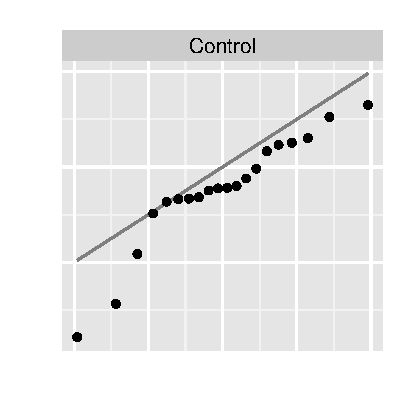
\includegraphics[width=0.3\textwidth]{qqplots1}
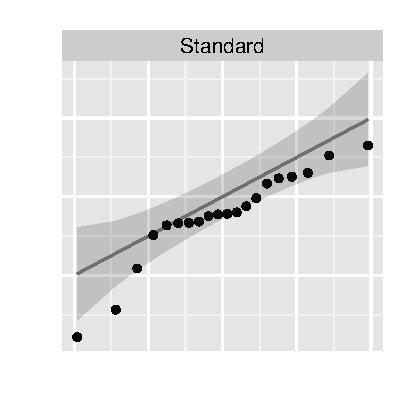
\includegraphics[width=0.3\textwidth]{qqplots2}
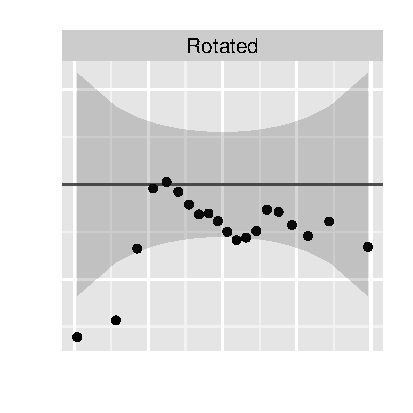
\includegraphics[width=0.3\textwidth]{qqplots3}
\caption{ \label{qqplots} Three versions of Q-Q plots: control, standard, and rotated.}
\end{figure}


Let $X_i \sim B_{1, \pi_i}, 1 \le i \le n$, where $X_i$ is the binary decision on the $i$th evaluation and $\pi_i$ is the probability with which the observer chooses the data plot. This probability is influenced by a number of factors:

\begin{center}
\begin{tabular}{lp{5in}}
$\tau$ & the design used in the lineup (Control, Standard, Rotated), \\
&  the specific parameters under which the data for the lineup was created: \\
&  $\delta$ \ \ \ degrees of freedom (2, 5, 10) {of the $t$ distribution} and \\
&  $\nu$  \ \ \ sample size (10, 20, 50, 75), \\
$d$ &  the level of difficulty based on the actual sample, and \\
$u$ & the users' subjective abilities.
 \end{tabular}
\end{center}
%
The above factors result in 12 different parameter settings. For each setting we created two samples, along with two sets of null data each, yielding 48 different lineups. 
Using  Amazon MTurk \citep{amazon}, 417 participants were each asked to evaluate ten different lineups. 
We model the probability of selecting the data plot from the lineup, $\pi$, with the help of model $M_1$:
\[
g(\pi_i) = \mu + \tau_{j(i)} +\delta_{k(i)}+ \nu_{s(i)} + u_{u(i)} + d_{d(i)}
\]
where $g$ is the logit link function, and $j(.), k(.), s(.), u(.)$, and $d(.)$ are all indexing functions that relate evaluation $i$ to the corresponding levels in the factor variables, to the observer, or a particular data sample. More specifically, $j(i) \in \{$Control, Standard, Rotated$\}$; $k(i) \in \{2,5,10\}$; $s(i) \in \{20, 30, 50, 75\}$; $u(i)$ maps to the participant's id of the $i$th evaluation and $d(i)$ identifies the particular data sample used for it. 

Both user ability, $u$, and sample difficulty, $d$, are modeled as independent, normally distributed  random effects, i.e. $u_{u(i)} \sim N(0, \sigma_u^2)$, $d_{d(i)} \sim N(0,\sigma_d^2)$ with cov$(u, d) = 0$.



%\begin{center}
%\begin{tabular}{lp{5.5in}}
%$\mu$ & overall mean\\
%$\tau_{j(i)}$ & is the effect of design $j$, $j \in \{ \text{Control, Standard, Rotated} \}$, and $j(i)$ is the design used in evaluation $i$, $1 \le i \le n$.  \\
%$\delta_{k(i)}$ & is the effect of $k$ degrees of freedom , $k \in \{ 2, 5, 10 \}$, and $k(i)$ is the degree of freedom used to generate the lineup  in evaluation $i$, $1 \le i \le n$.  \\
%$\nu_{\ell(i)}$ & is the effect of sample size $\ell$, $\ell \in \{ 20, 30, 50, 75 \}$, and $\ell(i)$ is the sample size used to generate the lineup  in evaluation $i$, $1 \le i \le n$.  \\
%$u_{u(i)}$ & user ability, $u_{u(i)} \sim N(0,1)$ i.i.d \\
%$d_{\ell(i)}$ & data difficulty, $d_{\ell(i)} \sim N(0,1)$ i.i.d 
%\end{tabular}
%\end{center}

% latex table generated in R 3.0.1 by xtable 1.7-1 package
% Sun May 26 13:36:30 2013
% xtable(summary(m0)@coefs, digits=c(0,2,3,2,4))
\begin{table}[ht]
\centering
\caption{\label{tab:model} Coefficients and significances corresponding to  model $M_1$. The type of design is important for the power of a lineup. Rotated Q-Q plots lose a significant amount of power compared to both the regular and the standard version of Q-Q plots. }
\begin{tabular}{rrrrrl}
  \hline
 &\bf Estimate &\bf Std. Error &\bf z value &\bf Pr($>$$|$z$|$) & \\ 
  \hline
Intercept & -5.04 & 0.769 & -6.55 & 0.0000 & *** \\ [3pt]
\multicolumn{3}{l}{\bf design} \\
   Control & 0.00 & ----- & ----- & ----- \\ 
   Rotated & -0.38 & 0.128 & -2.97 & 0.0030 & **\\ 
   Standard & 0.11 & 0.127 & 0.88 & 0.3782 \\ [3pt]
%  locationOuter & 0.19 & 0.106 & 1.83 & 0.0677 \\ 
%  clickSingle & -0.09 & 0.104 & -0.89 & 0.3747 \\ 
\multicolumn{4}{l}{\bf degrees of freedom} \\
  2 & 6.32 & 0.743 & 8.50 & 0.0000 & ***\\ 
  5 & 2.43 & 0.726 & 3.34 & 0.0008 & ***\\ 
  10 & 0.00 & ----- & ----- & ----- \\ [3pt]
\multicolumn{3}{l}{\bf sample size} \\
  20 & 0.00 & ----- & ----- & ----- \\ 
  30 & 1.09 & 0.844 & 1.29 & 0.1970 \\ 
  50  & 2.98 & 0.844 & 3.54 & 0.0004 & ***\\ 
  75 & 2.31 & 0.845 & 2.73 & 0.0063  & **\\ 
   \hline
\multicolumn{5}{l}{Signif. codes:  0 �***� 0.001 �**� 0.01 �*� 0.05 �.� 0.1 � � 1}
\end{tabular}
\end{table}

The estimated model coefficients for model $M_1$ are shown in Table~\ref{tab:model}. 
\hh{Estimates of the variance components are $\widehat{\sigma}_u = 0.71$, $\widehat{\sigma}_d=1.95$, and $\widehat{\sigma} = 0.29$. Variances of user ability and data difficulty are large relative to residual variance, indicating that both random effects are necessary.}
%
As expected, the task of identifying non-normality is easier with increased sample size and more pronounced deviations from normality, as is the case with lower degrees of freedom. The  design of the Q-Q plot is of huge importance for the probability of choosing the data plot. Interestingly, the rotated version of the Q-Q plot is significantly less suitable for the task of assessing normality compared to the control form. Adding confidence bands helps with evaluation, but not significantly. 

Note that none of the data plots in the lineups were actually created using data from a normal distribution. This should lead to rejection of the null hypothesis in every single instance. This is not quite true, as can be seen in Table~\ref{tab:reject}. But what also becomes evident is the high power  of visual inference. Based on lineups we are able to reject non-normality much more often than with any of the classical tests.

% latex table generated in R 3.0.1 by xtable 1.7-1 package
% Mon May 27 20:57:50 2013
\begin{table}[ht]
\centering
\caption{\label{tab:reject} 
Out of the 48 non-normal samples, 24 get rejected at the 5\% significance level based on evaluation by observers. None of the classical tests come close to that rejection rate. From left to right, we see the number of rejections from visual inference as well as the Anderson-Darling, Shapiro-Wilk, Cram\'er-von Mises and Kolmogorov-Smirnov tests for normality.}
\begin{tabular}{rrrrrr}
  \hline
Result & Visual & AD & SW & CVM & KS \\ 
  \hline
  reject & 24 & 10 & 16 &  8 & 10 \\ 
  not reject & 24 & 38 & 32 & 40 & 38 \\ 
   \hline
\end{tabular}
\end{table}

%------------------------------------------------------------------------------------
\section{Conclusion}\label{sec:conclusion}
%------------------------------------------------------------------------------------

We have presented a graphical approach to model selection and diagnosis based on simulating from the model fit to the true data. Use of the lineup protocol enables the creation of graphical tests, which enable not only the testing of hypotheses but subsequent exploration of the plots in the lineup to gain additional insight into the data structure. This approach relies only on the simulation process, graphics created, and observers recruited, avoiding the need to rely on asymptotic reference distributions; thus avoiding the pitfalls of many commonly used diagnostic tests. 
%It is important to note that simulation-based diagnostics for linear mixed-effects models have been discussed previously \citep{Longford:2001wy}, but graphical diagnosis was not the focus. A key advantage of the graphical approach is that fewer simulations are required, greatly reducing the computational burden of simulation-based diagnostics.

Throughout this paper we have provided examples of graphical diagnostics that we have found to be useful. Many situations, such as outlier detection, were not discussed in this paper. This omission was not because we overlooked these diagnostic situations, but because an exhaustive list is impossible. Based on the examples and discussion throughout this paper, and its predecessors, we believe the approach can be easily adapted.

Additionally, we have presented a more detailed look at graphical diagnostics that can be used to assess distributional assumptions. We found that, contrary to expectation, rotating the Q-Q plot to emphasize the vertical comparisons does not improve the power of the graphical test. In addition to supporting the use of the standard construction of Q-Q plots, this study provides an example of how to select a graphical diagnostic based on its estimated power. 

%\alnote{I'm not quite sure where to put this... We could add a paragraph here describing what was used, or maybe an appendix? If we put it here, should it be the last paragraph?}
%\hh{Technical implementation: R \citep{R} and packages for modeling lme4 \citep{lme4}, HLMdiag \citep{HLMDiag}, and visualizations ggplot2 \citep{ggplot2}, nullabor \citep{nullabor}, gridSVG \citep{gridSVG}. 
%Mahbub's website for experiments}

%------------------------------------------------------------------------------------
\paragraph{Acknowledgments}
%------------------------------------------------------------------------------------
We would like to thank Mahbubul Majumder, who conducted the Amazon MTurk study (\url{http://www.public.iastate.edu/~mahbub/}). R \citep{R} was used to implement all analyses and methods discussed in this paper: lme4 \citep{lme4} and HLMdiag \citep{HLMDiag} were used to model fitting and the calculation of diagnostic quantities, respectively, and ggplot2 \citep{ggplot2}, nullabor \citep{nullabor}, and gridSVG \citep{gridSVG} were used for visualization.
This work was funded in part by National Science Foundation grant DMS 1007697. All studies were conducted with approval from the internal review board IRB 10-347.

%------------------------------------------------------------------------------------
\appendix
\section{Data sets}
%------------------------------------------------------------------------------------

All of the data sets used in this paper are publicly available: the General Certificate of Secondary Education Exam data set is available in the R package mlmRev \citep{mlmRev}; the Dialyzer data set is available in the R package MEMSS \citep{MEMSS}; all other data sets can be found in the R package HLMdiag \citep{HLMDiag}.

\subsection{General certificate of secondary education exam data}\label{data:GCSE}

We make use of a subset of examination results of 4,065 students nested within 65 inner-London schools discussed by \cite{Goldstein:1993wm}. The original analysis explored school effectiveness as defined by students' performance on the General Certificate of Secondary Education (GCSEE) scores in both mathematics and English. This exam is taken the end of at the end of compulsory education, typically when students are 16 years old.  To adjust for a student's ability when they began secondary education, the students' scores on the standardized London Reading Test (LRT) and verbal reasoning group (bottom 25\%, middle 50\%, or top 25\%) at age 11. Additional information contained in the data set includes student gender, school gender, and the average LRT intake score for each school. 


\subsection{Autism study}\label{data:autism}
%------------------------------------------------------------------------------------
%\alnote{I need to pare this down.}
Autism is a developmental disorder typically characterized by impaired communication and social skills, but there is relatively little consensus on how these abilities or disabilities change over time \citep{Anderson:2007cl, Anderson:2009in}. 
In an effort to better understand changes in verbal and social abilities from childhood to adolescence \cite{Anderson:2007cl, Anderson:2009in} carried out a prospective longitudinal study following 214 children between the ages of 2 and 13 who had been diagnosed with either autism spectrum disorder or non-spectrum developmental delays at age 2. The Vineland Adaptive Behavior Interview survey was used to assess each child's interpersonal relationships, play time activities, and coping skills. This survey is completed by the parents. From the survey the Vineland Socialization Age Equivalent (VSAE) was computed as overall measure of a child's social skills. Additionally, expressive language development at age 2 was assessed using the Sequenced Inventory of Communication Development (SICD) and the children were classified into three groups (high, medium, or low). Assessments were made on the children ages 2, 3, 5, 9, and 13, however, not all children were assessed at each age. Additional information collected on each child includes: gender, race (white or non-white), and initial diagnosis at age 2 (autism, pervasive development disorder (pdd), or non-spectrum). We restrict attention to models concerned with the changes in social skills for subjects diagnosed with autism spectrum disorder having complete data. This results in a reduced data set of 155 children. For more detailed analyses we refer the reader to \cite{Anderson:2007cl, Anderson:2009in}.

\subsection{Methylprednisolone study}\label{data:ahd}
%------------------------------------------------------------------------------------

\cite{Carithers:1989} conducted a four week longitudinal study to investigate the effectiveness of methylprednisolone to treat patients with severe alcoholic hepatitis. The researchers randomly assigned 66 patients to receive either methylprednisolone (35 patients) or a placebo (31 patients). Over the study duration, each subject's serum bilirubin levels (in $\mu$mol/L) were measured each week, with the first measurement taken at the start of the study (week 0).

\subsection{Dialyzer study}\label{data:dialyzer}
%------------------------------------------------------------------------------------

\cite{Vonesh:1992us} describe a study characterizing the water transportation characteristics of 20 high flux membrane dialyzers, which were introduced to reduce the time a patient spends on hemodialysis. The 20 dialyzers were studied \emph{in vitro} using bovine blood at flow rates of either 200 or 300 ml/min, and the ultrafiltration rate (ml/hr) for each dialyzer was measured at seven transmembrane pressures (in mmHg). \cite{Vonesh:1992us} use nonlinear mixed-effects models to analyze these data; however, they can be modeled using polynomials in the linear mixed-effects framework.

\subsection{Radon study}\label{data:radon}
%------------------------------------------------------------------------------------

The data consist of a stratified random sample of 919 owener-occupied homes in 85 counties in Minnesota. For each home, a radon measurement was recorded (in log $pCi/L$, i.e., log picoCuries per liter) as well as a binary variable indicating whether the measurement was taken in the basement (0) or a higher level (1). Additionally, the average soil uranium content for each county was available. The number of homes within each county varies greatly between counties ranging from one home to 116 homes, with 50\% of counties having measurements from between 3 and 10 homes.\cite{Gelman:2006ue} suggest a simple hierarchical model allowing for a random intercept for each county and a random slope for floor level. This is the model from which we simulate predicted random effects.

%------------------------------------------------------------------------------------
\section{Additional lineups included in the study}
%------------------------------------------------------------------------------------

\begin{figure}
	\centering
	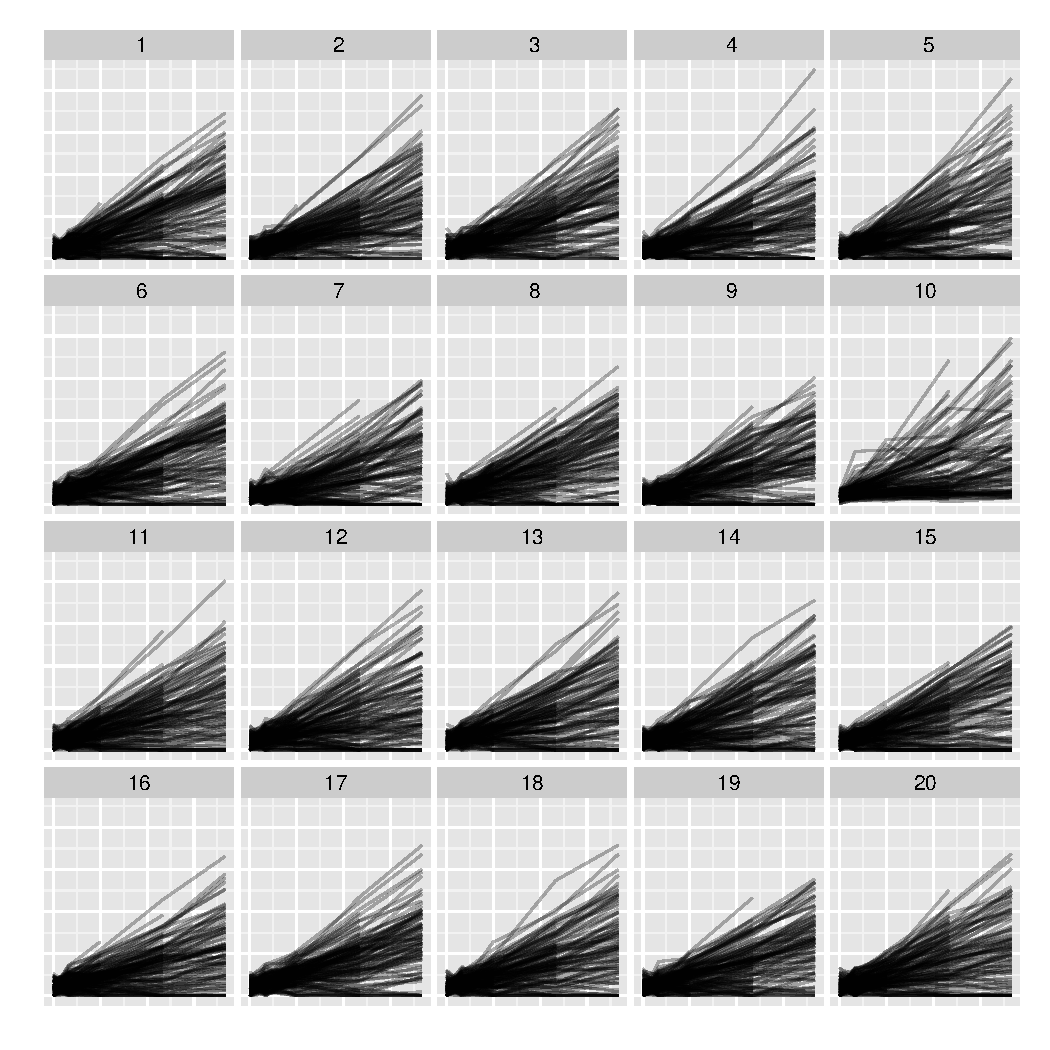
\includegraphics[width=\textwidth]{autism_ranef1_lineup10}
	\caption{\label{fig:autism-ranef} Which of the plots is the most different? Which feature led you to your choice? }
\end{figure}

\begin{figure}[h]
	\hfill
	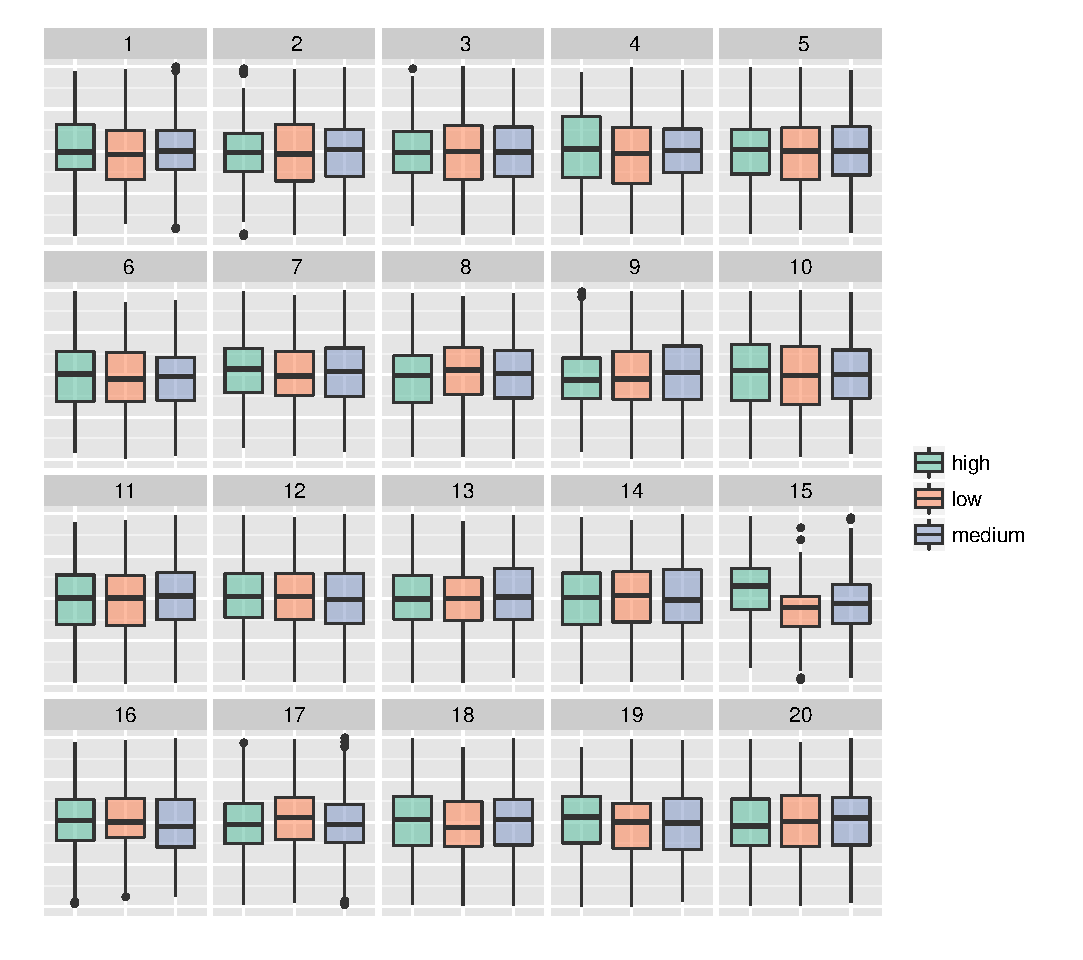
\includegraphics[width=0.9\textwidth]{autism_sicdegp_level1_lineup4.pdf}
	\caption{\label{fig:boxplot-unordered} An alternative layout of Figure~\ref{fig:boxplot-ordered}, where the boxplots are ordered as they are for inference. Which of the plots is the most different? Which feature led you to your choice?}
\end{figure}

\clearpage
%------------------------------------------------------------------------------------
%------------------------------------------------------------------------------------

\bibliographystyle{apalike}
\bibliography{hlmviz_bib}

\end{document}